% ---------------------------------------------------------------
% TEMPLATE TCC2 - SENAC SANTO AMARO
% ---------------------------------------------------------------
% Trabalho de Conclusão de Curso 2
% Elaborado para apresentação do trabalho final do TCC
% Estrutura: Introdução, Revisão Bibliográfica, Metodologia,
%            Desenvolvimento, Resultados e Análise, Conclusão
% ---------------------------------------------------------------

\documentclass[
    12pt,                % tamanho da fonte
    openright,           % capítulos começam em página ímpar
    oneside,             % para impressão em apenas um lado do papel
    a4paper,             % tamanho do papel
    english,             % idioma adicional
    brazil               % idioma principal
]{abntex2}

% ---------------------------------------------------------------
% PACOTES
% ---------------------------------------------------------------
\usepackage{lmodern}                % Fonte Latin Modern
\usepackage[T1]{fontenc}            % Seleção de códigos de fonte
\usepackage[utf8]{inputenc}         % Codificação do documento
\usepackage{lastpage}               % Usado pela Ficha catalográfica
\usepackage{indentfirst}            % Indenta o primeiro parágrafo
\usepackage{color}                  % Controle de cores
\usepackage{graphicx}               % Inclusão de gráficos
\usepackage{microtype}              % Melhorias de justificação
\usepackage{float}                  % Para posicionamento de figuras
\usepackage{booktabs}               % Tabelas profissionais
\usepackage{array}                  % Alinhamento das colunas p{} (Tabela do plano de experimentacao)
\usepackage{multirow}               % Células mescladas em tabelas
\usepackage{longtable}              % Tabelas longas
\usepackage{amsmath,amssymb}        % Símbolos matemáticos
\usepackage{pgfgantt}               % Diagramas de Gantt
\usepackage[brazilian,hyperpageref]{backref}  % Páginas com citações
\usepackage[alf]{abntex2cite}       % Citações ABNT

% ---------------------------------------------------------------
% CONFIGURAÇÕES DE APARÊNCIA DO PDF FINAL
% ---------------------------------------------------------------
\definecolor{blue}{RGB}{41,5,195}

% ---------------------------------------------------------------
% TAMANHO DA FONTE DAS LEGENDAS (ABNT) -- 10 pt
% ---------------------------------------------------------------
% O título (\caption) e a linha de fonte (\legend) de figuras e
% tabelas devem ficar em 10 pt (o corpo do texto é 12 pt). Por
% padrão o memoir/abntex2 deixa essas legendas em 12 pt; os comandos
% abaixo reduzem o título e a fonte para 10 pt.
\renewcommand{\ABNTEXfontereduzida}{\fontsize{10}{12}\selectfont}
\captionnamefont{\ABNTEXfontereduzida}   % rótulo "Figura N"/"Tabela N"
\captiontitlefont{\ABNTEXfontereduzida}  % texto do título da legenda
\makeatletter
% Redefine \legend (usado em "Fonte: ...") para sair em 10 pt
% (a definição original do memoir fixa \normalsize = 12 pt).
\renewcommand{\legend}[1]{%
  \M@gettitle{#1}%
  \memlegendinfo{#1}%
  \par
  \begingroup
    \@parboxrestore
    \if@minipage
      \@setminipage
    \fi
    \ABNTEXfontereduzida
    \captiondelim{\mbox{}}%
    \@makecaption{}{\ignorespaces #1}\par
  \endgroup}
\makeatother

% ---------------------------------------------------------------
% INFORMAÇÕES DO DOCUMENTO
% ---------------------------------------------------------------
\titulo{Avaliação de estratégias de treinamento com YOLOv8 para detecção de defeitos pequenos em cartas Pokémon TCG com baixo volume de dados}
\autor{Matheus da Silva Marini}
\local{São Paulo}
\data{2026}
\orientador{Prof. Afonso César Lelis Brandão}
% \coorientador{Prof. Nome do Coorientador} % Descomente se houver coorientador

\instituicao{%
  SENAC -- Serviço Nacional de Aprendizagem Comercial
  \par
  Unidade Santo Amaro
  \par
  Curso de Ciência da Computação
}

\tipotrabalho{Trabalho de Conclusão de Curso II}

\preambulo{Trabalho de Conclusão de Curso II apresentado ao SENAC Santo Amaro como requisito parcial para conclusão do curso de Ciência da Computação.}

% ---------------------------------------------------------------
% CONFIGURAÇÕES DO PDF
% ---------------------------------------------------------------
\makeatletter
\hypersetup{
    pdftitle={Avaliação de estratégias de treinamento com YOLOv8 para detecção de defeitos pequenos em cartas Pokémon TCG com baixo volume de dados},
    pdfauthor={Matheus da Silva Marini},
    pdfsubject={TCC2 - SENAC Santo Amaro},
    pdfcreator={LaTeX with abnTeX2},
    pdfkeywords={tcc2}{senac}{santo amaro}{trabalho de conclusão},
    colorlinks=true,        % false: links em caixas; true: links coloridos
    linkcolor=blue,         % cor dos links internos
    citecolor=blue,         % cor dos links para bibliografia
    filecolor=magenta,      % cor dos links para arquivos
    urlcolor=blue,
    bookmarksdepth=4
}
\makeatother


% ---------------------------------------------------------------
% COMPILA O ÍNDICE
% ---------------------------------------------------------------
\makeindex

\begin{document}

% ---------------------------------------------------------------
% ELEMENTOS PRÉ-TEXTUAIS
% ---------------------------------------------------------------
\pretextual

\imprimircapa

\imprimirfolhaderosto

% ---------------------------------------------------------------
% RESUMO
% ---------------------------------------------------------------
\begin{resumo}
Este trabalho avaliou o impacto de diferentes estratégias de
treinamento aplicadas ao YOLOv8 na detecção de defeitos superficiais em
cartas Pokémon TCG (\textit{Trading Card Game}). O objetivo foi
identificar quais combinações apresentam melhor desempenho com um
conjunto limitado de imagens. A escolha do tema baseou-se na escassez
de estudos que avaliam sistematicamente essas estratégias no domínio de
cartas colecionáveis. Nesse domínio, a graduação avalia a condição
física de cada exemplar, mas a inspeção manual é lenta e sujeita à
subjetividade do avaliador. Essas limitações motivam a sua automação
por visão computacional. A anotação de defeitos, porém, é cara, e a
busca bibliográfica realizada não identificou conjuntos de dados
públicos de cartas Pokémon TCG com defeitos localizados. Nos
experimentos, o modelo partiu de um YOLOv8s com \textit{transfer
learning} a partir de pesos pré-treinados no conjunto público de imagens COCO. Quatro configurações cruzaram o
uso ou não de aumento de dados com duas representações de entrada:
imagens RGB convencionais e imagens de realce de micro-relevo. Sobre a
configuração de melhor desempenho, avaliou-se o efeito de uma cabeça de
detecção adicional para objetos pequenos (P2) e da resolução de
entrada. O conjunto de dados reuniu 206 cartas, 412 imagens e 4.808
anotações, parte delas sugerida por modelos de uma etapa preliminar e
validada pelo autor. O desempenho foi medido pelo mAP@0,5, pela precisão, pela
revocação e pelo F1, em validação cruzada com cinco dobras. O F1 dá uma
única nota por carta, o que permitiu comparar as configurações carta a
carta pelo teste de Wilcoxon pareado, com correção de Holm. O aumento
de dados melhorou o detector: a Configuração 2, com imagens RGB e
aumento de dados, obteve o melhor desempenho, com F1 por carta de
0,376, contra 0,332 da mesma configuração sem aumento de dados. O
realce de micro-relevo foi inferior ao RGB quando não havia aumento de
dados. Com aumento de dados, essa diferença desapareceu quando a
avaliação desconsiderou as anotações sugeridas por esses modelos.
A cabeça P2 apresentou desempenho inferior à configuração vencedora,
com a mesma revocação e menor precisão. Essa variante não partiu de
pesos pré-treinados na cabeça de detecção nem em parte das camadas
intermediárias, e por isso o efeito isolado da cabeça P2 não pôde ser
separado da ausência de pré-treino. Em uma dobra avaliada (45 cartas),
aumentar a resolução de entrada de 640 para 1280 pixels elevou o
mAP@0,5 de 0,156 para 0,309 e o F1 por carta de 0,266 para 0,399;
esta última diferença foi confirmada pelo teste de Wilcoxon pareado.
Uma curva de aprendizado com intervalo de confiança por
\textit{bootstrap}, em duas dobras, mostrou que o desempenho ainda não havia estabilizado com o volume de dados
disponível. A evidência do aumento de dados vem de cinco dobras, e a da
resolução de entrada, de uma só. Por isso, com poucos dados, o aumento
de dados melhorou o detector nas duas representações de entrada, e a
maior resolução de entrada também o melhorou, mas com evidência mais
limitada. O realce de micro-relevo não trouxe ganho.

\vspace{\onelineskip}

\noindent
\textbf{Palavras-chave}: Visão Computacional. Detecção de Defeitos.
Pokémon TCG. Conjuntos de Dados Reduzidos. YOLOv8. Realce de Micro-Relevo.
\end{resumo}

% ---------------------------------------------------------------
% ABSTRACT -- OBRIGATÓRIO NO TCC2 (NBR 14724)
% ---------------------------------------------------------------
\begin{resumo}[Abstract]
 \begin{otherlanguage*}{english}
   This work evaluated the impact of different training strategies
   applied to YOLOv8 on the detection of surface defects in Pokémon TCG
   (\textit{Trading Card Game}) cards. The objective was to identify
   which combinations perform best with a limited set of images. The
   choice of topic was based on the scarcity of studies that
   systematically evaluate these strategies in the domain of
   collectible cards. In this domain, grading assesses the physical
   condition of each item, but manual inspection is slow and subject
   to the evaluator's subjectivity. These limitations motivate its
   automation through computer vision. Defect annotation, however, is
   expensive, and the bibliographic search carried out did not
   identify public datasets of Pokémon TCG cards with localized
   defects. In the experiments, the model started from a YOLOv8s with \textit{transfer learning} from
   weights pre-trained on the public COCO image dataset. Four
   configurations crossed the use or not of data augmentation with two
   input representations: conventional RGB images and micro-relief
   enhancement images. On top of the best-performing configuration,
   the effect of an additional detection head for small objects (P2)
   and of the input resolution was also evaluated. The dataset
   comprised 206 cards, 412 images, and 4,808 annotations, part of
   them suggested by models from a preliminary stage and validated by
   the author.
   Performance was measured by mAP@0.5, precision, recall and F1, in
   five-fold cross-validation. F1 gives a single score per card, which
   allowed the configurations to be compared card by card using a
   paired Wilcoxon test with Holm correction. Data augmentation improved
   the detector: Configuration 2, with RGB images and data augmentation,
   achieved the best performance, with a per-card F1 of 0.376, against
   0.332 for the same configuration without data augmentation.
   Micro-relief enhancement was inferior to RGB when there was no data
   augmentation. With data augmentation, this difference disappeared
   when the evaluation disregarded the annotations suggested by these
   models. The P2 head presented lower performance than the
   winning configuration, with the same recall and lower precision.
   This variant did not start from pre-trained weights in the detection
   head or in part of the intermediate layers, so the isolated effect
   of the P2 head could not be separated from the lack of pre-training.
   In one evaluated fold (45 cards), increasing the input resolution
   from 640 to 1280 pixels raised mAP@0.5 from 0.156 to 0.309 and the
   per-card F1 from 0.266 to 0.399; the latter difference was confirmed
   by the paired Wilcoxon test. A learning curve with a bootstrap confidence interval, over two folds,
   showed that performance had not yet stabilized with the available
   data volume. The evidence for data augmentation comes from five
   folds, and that for input resolution from only one. Therefore, with
   limited data, data augmentation improved the detector in both input
   representations, and higher input resolution also improved it, but with more limited
   evidence. Micro-relief enhancement brought no gain.

   \vspace{\onelineskip}

   \noindent
   \textbf{Keywords}: Computer Vision. Defect Detection. Pokémon TCG.
   Small Datasets. YOLOv8. Micro-Relief Enhancement.
 \end{otherlanguage*}
\end{resumo}

% ---------------------------------------------------------------
% LISTA DE ILUSTRAÇÕES (FIGURAS)
% ---------------------------------------------------------------
% Gerada automaticamente a partir das \caption{} das figuras.
% Toda figura com legenda passa a constar nesta lista.
\pdfbookmark[0]{\listfigurename}{lof}
\listoffigures*
\cleardoublepage

% ---------------------------------------------------------------
% LISTA DE TABELAS
% ---------------------------------------------------------------
% Gerada automaticamente a partir das \caption{} das tabelas.
\pdfbookmark[0]{\listtablename}{lot}
\listoftables*
\cleardoublepage

% ---------------------------------------------------------------
% LISTA DE ABREVIATURAS E SIGLAS
% ---------------------------------------------------------------
\pdfbookmark[0]{Lista de Abreviaturas e Siglas}{loas}
\chapter*{Lista de Abreviaturas e Siglas}

\noindent A lista a seguir reúne, em ordem alfabética, as abreviaturas e siglas utilizadas neste trabalho, acompanhadas de seus respectivos significados.

\vspace{\onelineskip}

\begin{center}
\begin{tabular}{@{}p{3.2cm}p{0.6\textwidth}@{}}
\toprule
\textbf{Abreviatura/Sigla} & \textbf{Significado} \\
\midrule
ACE    & \textit{Automatic Color Equalization} (Equalização Automática de Cor) \\
AMD    & \textit{Advanced Micro Devices} (fabricante da placa de vídeo usada nos experimentos) \\
AP     & \textit{Average Precision} (Precisão Média) \\
AVI    & \textit{Automated Visual Inspection} (Inspeção Visual Automatizada) \\
C2f    & \textit{Cross Stage Partial Bottleneck with two Convolutions} (módulo convolucional do YOLOv8) \\
CIELAB & Espaço de cor definido pela \textit{Commission Internationale de l'Éclairage}, com um canal de luminosidade (L$^*$) e dois de cor (a$^*$, b$^*$) \\
CLAHE  & \textit{Contrast Limited Adaptive Histogram Equalization} \\
CNN    & \textit{Convolutional Neural Network} (Rede Neural Convolucional) \\
COCO   & \textit{Common Objects in Context} \\
FN     & \textit{False Negative} (Falso Negativo) \\
FP     & \textit{False Positive} (Falso Positivo) \\
FPN    & \textit{Feature Pyramid Network} (Rede de Pirâmide de Características) \\
GPU    & \textit{Graphics Processing Unit} (Unidade de Processamento Gráfico) \\
HSV    & \textit{Hue, Saturation, Value} (Matiz, Saturação, Valor) \\
IoU    & \textit{Intersection over Union} \\
mAP    & \textit{mean Average Precision} (Média das Precisões Médias) \\
P1--P5 & Níveis da pirâmide de características do YOLOv8, numerados pela etapa de redução da imagem; no nível P$k$, o passo é de $2^k$ pixels (P1 = passo 2 a P5 = passo 32) \\
PANet  & \textit{Path Aggregation Network} \\
PSA    & \textit{Professional Sports Authenticator} \\
R-CNN  & \textit{Region-based Convolutional Neural Network} (Rede Neural Convolucional Baseada em Regiões) \\
RGB    & \textit{Red, Green, Blue} \\
ROCm   & \textit{Radeon Open Compute} (plataforma da AMD para executar computação em placas de vídeo) \\
SENAC  & Serviço Nacional de Aprendizagem Comercial \\
TCC    & Trabalho de Conclusão de Curso \\
TCG    & \textit{Trading Card Game} (Jogo de Cartas Colecionáveis) \\
TL     & \textit{Transfer Learning} \\
TP     & \textit{True Positive} (Verdadeiro Positivo) \\
UAV    & \textit{Unmanned Aerial Vehicle} (Veículo Aéreo Não Tripulado) \\
YOLO   & \textit{You Only Look Once} \\
\bottomrule
\end{tabular}
\end{center}

\cleardoublepage

% ---------------------------------------------------------------
% SUMÁRIO
% ---------------------------------------------------------------
\pdfbookmark[0]{\contentsname}{toc}
\tableofcontents*
\cleardoublepage

% ---------------------------------------------------------------
% ELEMENTOS TEXTUAIS
% ---------------------------------------------------------------
\textual

% ===============================================================
% CAPÍTULO 1 - INTRODUÇÃO
% ===============================================================
\chapter{Introdução}
\label{cap:introducao}

\textit{Trading Card Games} (TCG) são jogos de cartas colecionáveis nos quais
cada carta possui atributos únicos, como raridade, ilustração, edição, 
condição física e valor comercial. Além de sua função no contexto do 
jogo, essas cartas são negociadas entre jogadores e colecionadores, 
o que contribui para a formação de um mercado voltado à compra, venda, 
troca e avaliação de exemplares.
Representado por franquias como Pokémon e Magic: The 
Gathering, esse mercado deve movimentar aproximadamente 20 bilhões de 
dólares globalmente em 2026, com projeção de ultrapassar 76 bilhões 
até 2035 \cite{BRI2026}. Nesse contexto, o valor comercial de uma carta 
está diretamente ligado ao seu estado de conservação física. Para 
certificar essa condição e conferir segurança às transações, 
consolidou-se o serviço especializado de graduação de cartas 
(\textit{card grading}), no qual profissionais avaliam cada exemplar 
segundo critérios padronizados e atribuem uma nota que sintetiza sua 
qualidade \cite{Nahar2025}. A PSA (\textit{Professional Sports 
Authenticator}), pioneira nessa padronização, estabeleceu uma escala 
de 10 pontos que se tornaria norma do setor \cite{Nahar2025}, enquanto
a Beckett Grading Services atribui, além da nota geral, subnotas para
quatro atributos da carta, centralização, cantos, bordas e superfície,
ampliando o detalhamento do processo de avaliação \cite{Beckett_Standards}.

O processo de graduação, no entanto, ainda é realizado de forma
predominantemente manual. Os avaliadores inspecionam cada carta com
auxílio de instrumentos ópticos, como microscópios, o que torna a
análise demorada, sujeita à subjetividade de cada profissional e
difícil de escalar para acompanhar a demanda. Além disso, o manuseio
durante a inspeção pode causar desgaste à própria carta. Em um mercado
no qual uma carta pode valer de poucos dólares a centenas de milhares,
conforme a raridade e o estado de conservação, a precisão dessa
avaliação tem papel crítico no preço \cite{Nahar2025, Nahar2025b}.

Como resposta a esses desafios, a automação baseada em visão 
computacional tem sido investigada como alternativa à inspeção manual. 
Na indústria de manufatura, sistemas de inspeção visual automatizada 
(\textit{Automated Visual Inspection} -- AVI) já empregam arquiteturas 
de \textit{Deep Learning} e Redes Neurais Convolucionais (CNNs) para 
detectar defeitos em superfícies com alta velocidade e reprodutibilidade 
\cite{Zheng2021}. A adaptação dessas abordagens ao contexto de cartas 
colecionáveis, contudo, não é direta: as características visuais 
particulares das cartas e as condições reais de captura introduzem 
desafios técnicos específicos que limitam a transferência imediata 
das soluções desenvolvidas para domínios industriais convencionais 
\cite{Nahar2025}.

Um obstáculo adicional diz respeito à disponibilidade de dados. Em 
tarefas de detecção de objetos em domínios especializados, a construção 
de conjuntos de dados anotados em larga escala é custosa e trabalhosa, 
pois cada imagem exige rotulagem especializada com caixas delimitadoras 
precisas para cada instância de defeito \cite{Situ2023}. No contexto de cartas TCG, 
essa restrição é ainda mais pronunciada: a anotação requer avaliação especializada 
de defeitos segundo critérios técnicos de graduação, e o principal estudo identificado no domínio, conduzido sobre cartas esportivas, contou
com o apoio de um parceiro da indústria para viabilizar seu conjunto de dados
\cite{Nahar2025}.

Pesquisadores já investigaram o uso de técnicas de visão computacional
para classificar defeitos em cartas colecionáveis \cite{Nahar2025}, porém ainda há uma carência de estudos que avaliem
sistematicamente o impacto de diferentes estratégias de treinamento em
cenários com baixo volume de dados nesse domínio específico. Durante a
busca bibliográfica deste trabalho não foi identificado um conjunto de
dados público de imagens de cartas Pokémon TCG com os defeitos
localizados por caixas delimitadoras. O único conjunto público
encontrado difere do necessário neste trabalho em dois pontos: reúne
cartas esportivas, e não cartas Pokémon TCG, e traz recortes rotulados
para classificação, sem a posição de cada defeito \cite{Nahar2025b}.
Isso reforça a necessidade de construção de um conjunto próprio. Diante
disso, este trabalho realizou uma análise comparativa de estratégias de
treinamento para detecção de defeitos em cartas Pokémon TCG, conduzida
sobre um conjunto de dados composto por 206 cartas fornecido por uma
empresa brasileira especializada em graduação. Sobre um YOLOv8s com
\textit{transfer learning} a partir de pesos pré-treinados no conjunto
COCO, foram avaliados o aumento de dados (\textit{data augmentation}) e
o realce de micro-relevo (uma transformação da imagem que destaca
variações locais de intensidade associadas ao relevo da superfície,
como vincos e amassados) como representação de entrada. Essas duas estratégias foram cruzadas em um estudo fatorial,
que resultou em quatro configurações comparadas entre si. Em seguida,
sobre a configuração de melhor desempenho nessa comparação, foram
avaliadas uma cabeça de detecção adicional para objetos pequenos (P2) e
a resolução de entrada de 1280 pixels, em comparação com a resolução
padrão de 640 pixels. A avaliação foi realizada por meio de métricas
quantitativas consolidadas na literatura, com o objetivo de identificar
as combinações mais eficazes em cenários com dados limitados.

% ---------------------------------------------------------------
\section{Contextualização do problema}
\label{sec:contextualizacao}

Na graduação de cartas colecionáveis, a avaliação segue critérios 
físicos padronizados que consideram superfície, bordas, cantos e 
centralização como atributos independentes, cada um passível de 
apresentar tipos específicos de defeito \cite{Nahar2025}. Do ponto de 
vista visual, esses defeitos tendem a ser localizados em regiões 
específicas da carta e podem ocupar áreas reduzidas da imagem, o que 
os torna difíceis de identificar tanto manualmente quanto por meio de 
modelos computacionais \cite{Nahar2025}.

Do ponto de vista computacional, a detecção desses defeitos apresenta desafios
semelhantes aos encontrados em inspeção industrial automatizada, mas agravados
pelas características específicas das cartas TCG. O primeiro deles é a iluminação
durante a captura das imagens: quando a iluminação não produz bom
contraste entre o defeito e o fundo, ou quando introduz ruído na imagem,
o reconhecimento de defeitos por métodos supervisionados se torna mais
difícil \cite{Zheng2021}. No contexto de cartas colecionáveis, esse
efeito pode ser intensificado pela presença de artes visualmente complexas,
superfícies holográficas e defeitos de baixa visibilidade. Para mitigar seu impacto sobre a detecção de defeitos sutis,
operadores de filtragem têm sido aplicados como etapa de
pré-processamento em sistemas de inspeção visual
\cite{Sawada2024, Jiang2023}.

O segundo desafio são os reflexos em superfícies holográficas
(\textit{foil}). Em superfícies altamente refletoras, artefatos de
reflexo podem mascarar as características visuais necessárias para
identificar defeitos \cite{KimMG2026}. De modo análogo, o brilho da
superfície holográfica pode reduzir o contraste entre o defeito e a
região ao redor, e reflexos e sombras já são reconhecidos como fonte de
problema na captura de imagens de cartas \cite{Nahar2025}. Entre as estratégias avaliadas
neste trabalho, o realce de micro-relevo aumenta o contraste local da
imagem e pode atenuar em parte essa perda de contraste; nenhuma delas,
porém, atua sobre a captura da imagem, etapa em que o reflexo se forma.

Um terceiro desafio diz respeito à natureza da tarefa de inspeção em si.
Abordagens de classificação atribuem um rótulo à imagem, ou a um recorte
dela, como um canto da carta, sem fornecer informação sobre a
localização do defeito \cite{Hussain2023}. Um canto pode apresentar
\textit{whitening} restrito à sua extremidade, mas o classificador
produz apenas uma nota global para aquela região, sem indicar a posição
ou a extensão do dano. Quando essa informação é necessária, a detecção
de objetos, que localiza cada instância por caixa delimitadora e lhe
atribui uma classe \cite{Ramos2025}, é apontada como preferível à
classificação de imagens em inspeção de defeitos \cite{Hussain2023}.
Neste trabalho, a detecção foi conduzida com uma única classe,
denominada \textit{defeito}: o modelo localiza cada instância, mas não
distingue o tipo de defeito nem sua gravidade. Mesmo sem essas
informações, a localização tem valor próprio, pois indica ao avaliador
em que pontos da carta concentrar a inspeção.

Um quarto desafio diz respeito ao tamanho dos defeitos. Antes de entrar
na rede, a imagem é redimensionada para a resolução de entrada: na
resolução de 640 pixels, por exemplo, ela é redimensionada, mantendo a
proporção, até que seu lado maior meça 640 pixels. A rede, por sua vez,
reduz essa imagem em etapas, e cada nível de detecção trabalha sobre um
mapa de características em que um único ponto resume um bloco de pixels
da imagem de entrada; o lado desse bloco é chamado de passo. No nível de
passo 8, por exemplo, cada ponto resume um bloco de 8 $\times$ 8
pixels, e o sinal de um defeito cujo menor lado é menor que 8 pixels
ocupa só uma parte de cada bloco em que aparece e fica diluído no ponto
que resume esse bloco. Na resolução de entrada de 640 pixels, que é a
resolução padrão do YOLOv8, 57,6\% dos defeitos deste conjunto de dados
têm o menor lado da caixa delimitadora abaixo de 8 pixels, o passo do
nível de detecção mais fino do YOLOv8 original (P3); essa proporção cai
para 10,8\% quando a resolução de entrada sobe para 1280 pixels. Essa
restrição motivou a avaliação de uma cabeça de detecção adicional
voltada a objetos pequenos (P2, de passo 4) e da resolução de entrada
como estratégias deste trabalho.

Por fim, a construção de conjuntos de dados anotados nesse domínio
impõe restrições práticas que delimitam diretamente o escopo de
investigação possível. Mesmo o principal estudo identificado no domínio
trabalhou com um conjunto que os próprios autores caracterizam como
pequeno \cite{Nahar2025}, o que evidencia por que cenários com poucos
exemplos rotulados constituem uma restrição real que demanda
estratégias de treinamento específicas. Um sistema integrado de
graduação automática, apresentado por seus autores como pronto para uso
em produção, avalia cantos, bordas e superfície de forma unificada, com
algumas centenas de cartas (593 para cantos, 134 para bordas e 150 para
superfície) \cite{Nahar2025b}. Esse sistema, porém, classifica recortes
da carta, sem localizar os defeitos na imagem. A diferença para este
trabalho é, portanto, sobretudo de tarefa: aqui, o modelo
detecta cada defeito e o localiza por caixa delimitadora.

% ---------------------------------------------------------------
\section{Formulação do problema}
\label{sec:formulacao}

Diante desses desafios, o problema investigado neste trabalho pode ser
formulado pela seguinte pergunta: com um conjunto reduzido de imagens
anotadas, quais estratégias de treinamento aplicadas ao YOLOv8, entre
aumento de dados, realce de micro-relevo como representação de entrada,
cabeça de detecção adicional para objetos pequenos e resolução de
entrada, melhoram a detecção de defeitos superficiais em cartas
Pokémon TCG? O trabalho restringe-se à detecção de defeitos com uma
classe única, sem atribuir a nota de graduação da carta, e à
comparação dessas estratégias sobre um mesmo conjunto de dados e um
mesmo protocolo de avaliação.

As anotações de defeito usadas neste trabalho foram feitas por um único
anotador, o próprio autor, com apoio nos laudos de graduação emitidos
pela empresa que forneceu o conjunto de dados e no próprio julgamento
sobre a imagem, inclusive para defeitos não registrados nesses laudos.
A referência contra a qual o detector é medido é, portanto, o
julgamento desse anotador apoiado nos laudos, e não o laudo em si; sem
um segundo anotador, não foi possível medir a concordância entre
avaliadores, e o desempenho que é possível medir fica limitado pela
consistência dessa anotação. Parte das caixas delimitadoras, 892 de
4.808 (18,6\%), foi sugerida por modelos de detecção treinados em uma
etapa preliminar do trabalho e validada individualmente pelo autor, em
uma revisão da anotação descrita na Seção~\ref{subsec:dados}. Esses
modelos usavam imagens coloridas convencionais (RGB), com aumento de
dados, e nenhum deles havia sido treinado com a carta para a qual
sugeriu caixas. Como esses modelos viam as imagens da mesma forma que as
configurações que usam imagens RGB, as caixas sugeridas podem favorecer
essas configurações na comparação com o realce de micro-relevo; por
esse motivo, os resultados apresentados no
Capítulo~\ref{cap:desenvolvimento} foram verificados também
desconsiderando essas caixas sugeridas.

% ---------------------------------------------------------------
\section{Objetivos e hipótese}
\label{sec:objetivos}

Os objetivos a seguir decorrem da lacuna e da restrição apresentadas
nas seções anteriores: há carência de estudos que avaliem
sistematicamente estratégias de treinamento para detectar defeitos em
cartas colecionáveis, e o conjunto de dados disponível reúne apenas 206
cartas. Por isso, o objetivo é comparativo: em vez de propor um modelo
novo, o trabalho avalia quais estratégias melhoram um detector já
estabelecido, o YOLOv8, nesse cenário.

\subsection{Objetivo geral}

Avaliar o desempenho de estratégias de treinamento aplicadas ao modelo YOLOv8 para detecção de defeitos pequenos em cartas Pokémon TCG com baixo volume de dados.

\subsection{Objetivos específicos}

Para alcançar o objetivo geral, foram definidos os seguintes objetivos específicos:

\begin{enumerate}
    \item Organizar e preparar um conjunto de dados de imagens de cartas 
    Pokémon TCG, adotando uma classe única de detecção denominada 
    \textit{defeito}.
    
    \item Implementar quatro configurações experimentais baseadas em YOLOv8 com
    \textit{transfer learning}, cruzando o uso de aumento de dados
    (\textit{data augmentation}) com duas representações de entrada,
    imagens RGB convencionais e imagens de realce de micro-relevo, e
    comparar as quatro combinações resultantes.

    \item Avaliar, sobre a configuração de melhor desempenho nessa
    comparação, o efeito de uma cabeça de detecção adicional voltada a
    objetos menores (P2), pela revocação (a proporção dos defeitos
    anotados que o modelo encontra) dos defeitos cujo menor lado da
    caixa delimitadora é menor que 8 pixels, e o efeito da resolução de
    entrada, comparando 1280 e 640 pixels pelo F1 por carta, com teste
    de Wilcoxon pareado.

    \item Comparar o desempenho das diferentes configurações por meio
    de métricas quantitativas consolidadas em detecção de objetos,
    incluindo precisão (\textit{Precision}), revocação (\textit{Recall}),
    F1-\textit{score} e \textit{mean Average Precision} (mAP@0,5).

    \item Avaliar, por meio de uma curva de aprendizado, se o desempenho
    do detector aumenta com o número de cartas disponíveis para treino.

    \item Analisar os resultados obtidos, identificando quais estratégias
    de treinamento apresentam melhor desempenho em cenários com conjuntos
    de dados reais e limitados no domínio de inspeção de cartas TCG.
\end{enumerate}

\subsection{Hipótese ou critério de validação}
\label{subsec:hipotese}

A partir da revisão da literatura, foram formuladas as hipóteses H1 a
H3; a hipótese H4 foi formulada depois, a partir da análise do tamanho
das anotações apresentada na Seção~\ref{sec:contextualizacao}. As
quatro hipóteses foram formuladas antes do treinamento dos modelos
usados para testá-las:

\begin{description}
    \item[H1] O aumento de dados (\textit{data augmentation}) melhora o desempenho do detector em relação à configuração sem aumento de dados.
    \item[H2] O uso de imagens de realce de micro-relevo como representação de entrada melhora o desempenho do detector em relação às imagens RGB.
    \item[H3] A combinação de aumento de dados e realce de micro-relevo (Configuração 4) produz o melhor desempenho entre as quatro configurações avaliadas.
    \item[H4] A cabeça de detecção adicional P2 aumenta a revocação (\textit{recall}) dos defeitos cujo menor lado da caixa delimitadora é menor que 8 pixels, na resolução de entrada de 1280 pixels.
\end{description}

A métrica usada para testar H1 a H3 foi o F1 por carta, que resume em
um único valor a precisão e a revocação das detecções de cada carta;
seu cálculo é descrito no Capítulo~\ref{cap:desenvolvimento}. H1 foi testada pela comparação
pareada por carta entre a Configuração 2 (RGB com aumento de dados) e a
Configuração 1 (RGB sem aumento de dados), e entre a Configuração 4
(realce com aumento de dados) e a Configuração 3 (realce sem aumento de
dados). H2 foi testada pela comparação entre a Configuração 3 e a
Configuração 1, e entre a Configuração 4 e a Configuração 2. H3 seria
refutada se alguma das outras configurações superasse significativamente a Configuração 4, o que foi verificado pelas mesmas comparações da Configuração 4 com as Configurações 2 e 3, sem teste adicional; a regra completa de decisão das três hipóteses é apresentada no Capítulo~\ref{cap:desenvolvimento}. Todas essas comparações
usaram o teste de Wilcoxon pareado bilateral, com nível de
significância $\alpha = 0{,}05$, definido antes do treinamento das
quatro configurações; a correção de Holm para o conjunto de comparações foi
aplicada na análise dos resultados.

Para H4, o critério, definido antes do treinamento da variante com a
cabeça P2, foi a revocação dos defeitos cujo menor lado da caixa é
menor que 8 pixels na resolução de 1280 pixels, somados todos os
defeitos desse grupo, comparando a configuração de melhor desempenho
com e sem a cabeça P2. Mesmo nessa resolução, parte dos defeitos
permanece abaixo do passo do nível P3 (Seção~\ref{sec:contextualizacao}),
o que justificou testar a P2 nessa resolução. Já se sabia, antes desse
treinamento, que a variante com a cabeça P2 não receberia pesos
pré-treinados na cabeça de detecção nem em parte das camadas
intermediárias; por isso, o teste de H4 não separa o efeito da cabeça
P2 do efeito da falta de pré-treino.

A resolução de entrada e a curva de aprendizado foram análises
exploratórias, decididas depois dos resultados do estudo fatorial e sem
hipótese formulada previamente; seus resultados indicam direções a
confirmar. A confirmação ou a refutação de cada hipótese é apresentada
nos resultados e retomada na conclusão.

% ---------------------------------------------------------------
\section{Justificativa}
\label{sec:justificativa}

No âmbito científico, os estudos existentes sobre automação da
graduação de cartas colecionáveis apresentam contribuições relevantes, mas com
lacunas que abrem espaço para a investigação realizada neste trabalho.
\citeonline{Nahar2025} propõem um modelo baseado em \textit{transfer
learning} para classificar a severidade de defeitos em cantos,
alcançando 83\% de acurácia média em um conjunto de 4.744 imagens de
cantos obtidas de 593 cartas esportivas, mas o estudo está restrito a um único
critério de avaliação e não analisa sistematicamente o impacto de
diferentes estratégias de treinamento no desempenho do modelo.
Embora o sistema integrado descrito na
Seção~\ref{sec:contextualizacao} alcance acurácias de 81\% a 94\% na
classificação de recortes \cite{Nahar2025b}, a investigação
sistemática do impacto de estratégias de treinamento na detecção
localizada de defeitos, com conjuntos reduzidos de dados reais,
permanece uma lacuna no domínio de cartas colecionáveis, que este
trabalho investigou sobre um conjunto de 206 cartas e 412 imagens.

A relevância de investigar estratégias como
\textit{transfer learning} e aumento de dados em cenários
com amostras escassas é sustentada pela literatura de
inspeção visual automatizada. \citeonline{Chen2021}
identificam o problema de pequenas amostras
(\textit{small sample problem}) como um dos problemas
centrais da detecção de defeitos superficiais industriais com
aprendizado profundo, associado ao risco de sobreajuste, e
apontam quatro linhas de solução: aumento de dados, modelos
não supervisionados ou semissupervisionados,
\textit{transfer learning} e otimização da estrutura da rede.
Um exemplo quantitativo é apresentado por \citeonline{Wang2022},
na detecção de defeitos superficiais em aço: com apenas cinco
imagens rotuladas por categoria, pré-treinar o detector em
outras categorias de defeito antes do ajuste fino elevou o mAP
de 9,4\% para 24,1\%, em relação ao mesmo modelo treinado
somente com essas imagens. Nesse mesmo experimento, o aumento de
dados, uma das estratégias avaliadas neste trabalho, acrescentou até
2,3 pontos percentuais ao mAP.

Na prática, avaliar essas estratégias (aumento de dados, realce de
micro-relevo, a cabeça de detecção adicional P2 e a resolução de
entrada) sobre um YOLOv8s com \textit{transfer learning} a partir do
conjunto COCO indica quais delas merecem ser priorizadas quando o
volume de dados de treinamento é pequeno, um cenário comum em domínios
especializados como o de cartas colecionáveis. Um resultado negativo
(uma estratégia que não melhora o desempenho nesse cenário) também
constitui uma contribuição, pois evita que trabalhos futuros repitam o
mesmo investimento sem o ganho esperado. Essa análise é relevante para
contextos em que a anotação é cara e o volume de dados é limitado
\cite{Situ2023, Chen2021}, e busca subsidiar a detecção automática de
defeitos como apoio à inspeção visual \cite{Nahar2025}.

% ===============================================================
% CAPÍTULO 2 - REVISÃO BIBLIOGRÁFICA
% ===============================================================
\chapter{Revisão Bibliográfica / Trabalhos Relacionados}
\label{cap:revisao}

Este capítulo apresenta a pesquisa bibliográfica que fundamenta o
trabalho, os conceitos teóricos necessários para compreender os
experimentos e os trabalhos relacionados. A
Seção~\ref{sec:metodologia_pesquisa_bib} descreve como a literatura foi
buscada e selecionada. A Seção~\ref{sec:fundamentos} apresenta os
fundamentos, do geral para o específico. Começa pela base: aprendizado
profundo e redes neurais convolucionais, inspeção visual automatizada,
defeitos visuais em cartas colecionáveis, detecção de objetos, métricas
de avaliação de detectores e a arquitetura YOLO. Em seguida, trata do
\textit{transfer learning} usado em todos os experimentos, do cenário
com poucos dados e das estratégias avaliadas neste trabalho: aumento de
dados, realce de micro-relevo, cabeça de detecção adicional para
objetos pequenos e resolução de entrada. Por fim, apresenta os
conceitos usados para comparar essas estratégias: estudo fatorial e
estudo de ablação, validação cruzada e comparação estatística. A
Seção~\ref{sec:trabalhos_correlatos} analisa os trabalhos mais próximos
do problema investigado e indica como este trabalho se diferencia
deles.

% ---------------------------------------------------------------
\section{Metodologia da pesquisa bibliográfica}
\label{sec:metodologia_pesquisa_bib}

A pesquisa bibliográfica foi realizada por meio das bases Google Scholar, 
IEEE Xplore, ScienceDirect e MDPI, utilizando combinações de termos em 
inglês diretamente relacionados aos temas centrais do trabalho. As 
strings de busca utilizadas, bem como os quantitativos de artigos 
triados e selecionados em cada etapa, estão apresentados na 
Tabela~\ref{tab:strings_busca}. A triagem considerou título e resumo 
como critérios iniciais de relevância, com leitura completa reservada
aos trabalhos selecionados para inclusão. A busca ocorreu em duas fases:
uma exploratória, com strings temáticas, e outra dirigida, para
localizar a fundamentação de decisões de método específicas, como o
operador de realce, a comparação estatística e os critérios de
treinamento; por isso, parte das strings da
Tabela~\ref{tab:strings_busca} é mais específica que as demais.

% Bates2024 ficou FORA do texto (conferente, 26/10/2026): a frase do
% k = 5 usa só Arlot2010 e Kohavi1995. A triagem da busca do k (3
% triados a mais) foi somada à linha "cross-validation AND model
% selection AND survey" sem novo selecionado. Total de selecionados deve
% igualar o de chaves citadas.
\begingroup
\footnotesize
\begin{longtable}{p{7.5cm}|c|c|c}
\caption{Strings de busca utilizadas na pesquisa bibliográfica}
\label{tab:strings_busca} \\
\toprule
\textbf{String de busca} & \textbf{Bases} & \textbf{Triados} & \textbf{Selecionados} \\
\midrule
\endfirsthead
\toprule
\textbf{String de busca} & \textbf{Bases} & \textbf{Triados} & \textbf{Selecionados} \\
\midrule
\endhead
\bottomrule
\endfoot
\bottomrule
\endlastfoot
\textit{``trading card'' OR ``collectible card'' AND ``computer vision''}
    & GS, IEEE, SD, MDPI & 14 & 4 \\
\midrule
\textit{``surface defect detection'' AND ``computer vision'' AND ``scratch'' OR ``wear''}
    & GS, IEEE, SD, MDPI & 9 & 2 \\
\midrule
\textit{``PCB'' AND ``surface defect detection'' AND ``global contextual attention'' AND ``YOLO''}
    & GS, IEEE, SD, MDPI & 8 & 1 \\
\midrule
\textit{``ablation study'' AND ``object detection'' AND ``transfer learning''}
    & GS, IEEE, SD, MDPI & 5 & 2 \\
\midrule
\textit{``dataset COCO'' AND ``object detection'' AND ``YOLO pretraining''}
    & GS, IEEE, SD, MDPI & 3 & 1 \\
\midrule
\textit{``ImageNet pre-training'' AND ``from scratch'' AND ``object detection''}
    & GS, IEEE, SD, MDPI & 13 & 2 \\
\midrule
\textit{``filter'' AND ``surface defect detection'' AND ``deep learning''}
    & GS, IEEE, SD, MDPI & 18 & 3 \\
\midrule
\textit{``vessel enhancement'' AND ``Hessian'' AND ``multiscale''}
    & GS, IEEE, SD, MDPI & 5 & 1 \\
\midrule
\textit{``three-channel'' AND ``SAR'' AND ``YOLO'' AND ``ship detection''}
    & GS, IEEE, SD, MDPI & 4 & 1 \\
\midrule
\textit{``CLAHE'' AND ``transfer learning'' AND ``from scratch'' AND ``domain shift''}
    & GS & 3 & 1 \\
\midrule
\textit{``YOLOv8'' AND ``defect detection'' AND ``transfer learning''}
    & GS, IEEE, SD, MDPI & 11 & 4 \\
\midrule
\textit{``cross-validation'' AND ``YOLO'' AND ``defect detection''}
    & GS, IEEE, SD, MDPI & 6 & 1 \\
\midrule
\textit{``cross-validation'' AND ``model selection'' AND ``survey''}
    & GS, IEEE, SD, MDPI & 11 & 2 \\
\midrule
\textit{``statistical comparison'' AND ``classifiers'' AND ``cross-validation''}
    & GS, IEEE, SD, MDPI & 10 & 3 \\
\midrule
\textit{``bootstrap confidence intervals'' AND ``BCa''}
    & GS, IEEE, SD, MDPI & 14 & 2 \\
\midrule
\textit{``metric-related pitfalls'' AND ``image analysis'' AND ``validation''}
    & GS, IEEE, SD, MDPI & 2 & 1 \\
\midrule
\textit{``Neural Networks'' AND ``Early Stopping''}
    & GS, IEEE, SD, MDPI & 2 & 1 \\
\midrule
\textit{``learning curves'' AND ``deep networks'' AND ``analysis''}
    & GS, IEEE, SD, MDPI & 20 & 3 \\
\midrule
\textit{``small object detection'' AND ``input resolution'' OR ``image size''}
    & GS, IEEE, SD, MDPI & 9 & 3 \\
\midrule
\textit{``highly reflective'' surface defect detection YOLO}
    & MDPI & 9 & 1 \\
\midrule
Fontes não acadêmicas (contextualização de mercado e documentação técnica)
    & Diversas & n/a & 3 \\
\midrule
\textbf{Total} & & \textbf{176} & \textbf{42} \\
\end{longtable}
\endgroup
\legend{GS = Google Scholar; IEEE = IEEE Xplore; SD = ScienceDirect; MDPI = Multidisciplinary Digital Publishing Institute.
Fonte: Elaborado pelo autor (2026).}

Foram priorizados trabalhos acadêmicos publicados entre 2021 e 2026,
em língua inglesa, disponíveis em periódicos ou anais de conferências.
A seleção considerou principalmente estudos revisados por pares e
\textit{surveys} recentes quando diretamente relacionados ao problema
investigado ou necessários para fundamentar conceitos técnicos
específicos. Trabalhos anteriores a 2021 foram admitidos apenas quando
são a origem ou a referência clássica de um método, de um conjunto de
dados ou de um resultado empírico usado como fundamento neste trabalho, com alto impacto medido pelo número de citações no
OpenAlex, acima de mil em todos os casos na consulta de outubro de
2026; toda a literatura sobre detecção de defeitos e sobre o
domínio de cartas colecionáveis permaneceu restrita a 2021 em diante.
Por esse critério, foram incluídos nove trabalhos anteriores a 2021,
agrupados a seguir por tema; os conceitos mencionados são apresentados
na Seção~\ref{sec:fundamentos} e no Capítulo~\ref{cap:desenvolvimento}.
Como base de pré-treinamento, o conjunto
COCO \cite{Lin2014}, no qual foram obtidos os pesos iniciais do YOLOv8.
Em validação cruzada e seleção de modelos, \citeonline{Kohavi1995},
para a estratificação das dobras; \citeonline{Arlot2010}, para a
escolha do número de dobras; e \citeonline{Cawley2010}, para o viés de
fazer escolhas no mesmo conjunto usado para medir o desempenho. Em
comparação estatística, \citeonline{Demsar2006}, para o teste de
Wilcoxon pareado e a correção de Holm
(Seção~\ref{subsec:comparacao_estatistica}), e
\citeonline{DiCiccio1996}, para o intervalo de confiança por
\textit{bootstrap}. No treinamento, \citeonline{Prechelt1998}, para o
critério de parada antecipada adotado na
Seção~\ref{subsec:hiperparametros}, e \citeonline{He2019}, para o
efeito do pré-treino quando há poucos dados. Em processamento de
imagem, \citeonline{Frangi1998}, cuja medida foi usada no realce de
micro-relevo.

De forma complementar, também foram consultadas fontes não acadêmicas:
páginas institucionais e relatórios setoriais, utilizados para
contextualização do mercado e caracterização do domínio de aplicação
\cite{BRI2026,Beckett_Standards}, e a documentação técnica da biblioteca Ultralytics,
utilizada para os detalhes de implementação do YOLOv8 \cite{Jocher2023}.
A relevância de cada trabalho foi 
avaliada com base em sua aderência ao problema de pesquisa, isto é, a 
detecção automatizada de defeitos visuais em cenários com baixo volume 
de dados, com ênfase em aplicações de visão computacional em domínios 
especializados.




% ---------------------------------------------------------------
\section{Fundamentos teóricos}
\label{sec:fundamentos}
\label{sec:referencial}

Esta seção apresenta os conceitos teóricos que sustentam os
experimentos, organizados do geral para o específico. As
Seções~\ref{subsec:dl_cnn} a~\ref{subsec:yolo} tratam da base:
aprendizado profundo, inspeção visual automatizada, defeitos em cartas
colecionáveis, detecção de objetos, métricas de avaliação e a
arquitetura YOLO. As Seções~\ref{subsec:transfer_learning}
a~\ref{subsec:objetos_pequenos} tratam do cenário com poucos dados e
das estratégias avaliadas. As Seções~\ref{subsec:ablacao_conceito}
a~\ref{subsec:comparacao_estatistica} tratam de como essas estratégias
foram comparadas.

\subsection{Deep Learning e Redes Neurais Convolucionais}
\label{subsec:dl_cnn}

\textit{Deep Learning} é uma subárea do aprendizado de máquina que utiliza
redes neurais artificiais com múltiplas camadas para aprender representações
diretamente a partir dos dados. Em visão computacional, essa abordagem reduziu
a dependência de características projetadas manualmente, permitindo que os
modelos extraíssem padrões visuais complexos a partir das próprias imagens
\cite{Zheng2021}. Nesse contexto, as Redes Neurais Convolucionais (CNNs, do
inglês \textit{Convolutional Neural Networks}) tornaram-se a arquitetura central
para tarefas como classificação de imagens, detecção de objetos e inspeção de
defeitos, pois utilizam camadas convolucionais para aprender características
visuais em diferentes níveis de abstração \cite{Hussain2023}.

A relevância das CNNs em visão computacional foi consolidada por arquiteturas
como AlexNet, VGGNet, GoogLeNet, ResNet e DenseNet, que demonstraram a eficácia
de redes profundas na extração automática de características visuais
\cite{Zheng2021,Hussain2023}. Embora apresentem diferenças estruturais, essas
arquiteturas compartilham a ideia de aprender representações hierárquicas da
imagem, nas quais camadas iniciais capturam padrões simples, como bordas e
texturas, enquanto camadas mais profundas representam formas e estruturas mais
complexas.

Na inspeção visual automatizada, essa capacidade é especialmente importante
porque defeitos de superfície podem variar em forma, escala, textura e contraste.
Segundo \citeonline{Zheng2021}, métodos tradicionais dependiam de atributos
manualmente projetados, o que os tornava sensíveis a variações nas condições de
captura e no tipo de defeito. Já métodos baseados em \textit{deep learning}
integram a extração e a aprendizagem de características em um mesmo processo,
favorecendo maior adaptação a diferentes cenários de inspeção.

Essa base também sustenta arquiteturas modernas de detecção, como a família
YOLO, nas quais redes convolucionais são utilizadas para extrair características
visuais que posteriormente são empregadas na localização e classificação dos
objetos de interesse \cite{Hussain2023}. Assim, a compreensão das CNNs é
necessária para fundamentar o uso de detectores baseados em \textit{deep learning}
na identificação de defeitos visuais em cartas TCG.

\subsection{Visão Computacional e Inspeção Visual Automatizada}
\label{subsec:avi}

A visão computacional é a área da ciência da computação que desenvolve 
métodos para que sistemas digitais interpretem e analisem imagens e 
vídeos automaticamente. Uma de suas aplicações mais relevantes na prática 
industrial está nos sistemas de inspeção visual automatizada 
(\textit{Automated Visual Inspection} -- AVI), cuja função é substituir 
ou apoiar a inspeção manual de qualidade em linhas de produção 
\cite{Zheng2021}.

Um sistema AVI é composto, em geral, por três etapas principais: aquisição 
de imagem, detecção de defeitos e controle de qualidade. A etapa de 
aquisição utiliza câmeras digitais combinadas com sistemas de iluminação 
controlada para garantir contraste adequado entre as características do 
produto e possíveis defeitos. Em seguida, a etapa de detecção aplica 
algoritmos de processamento de imagem para identificar e classificar 
anomalias. Por fim, os resultados são enviados ao sistema de controle 
de qualidade, que determina a aceitação ou rejeição do produto 
\cite{Zheng2021}.

Antes da consolidação do \textit{Deep Learning}, muitos sistemas AVI 
dependiam de características projetadas manualmente por especialistas, 
o que os tornava sensíveis a variações nas condições de aplicação 
\cite{Zheng2021}. Com o avanço das CNNs, passaram a ser desenvolvidos 
métodos capazes de aprender padrões diretamente a partir dos dados de 
treinamento, superando parte das limitações dos métodos tradicionais. 
Sistemas baseados em CNNs têm sido avaliados na inspeção de defeitos
em semicondutores, aço e tecidos, e alguns estudos relatam acurácias de
classificação acima de 99\% em defeitos de aço e de placas de circuito
impresso \cite{Zheng2021}.

\subsection{Defeitos visuais em cartas colecionáveis}
\label{subsec:defeitos_visuais}

A inspeção visual de cartas colecionáveis envolve a identificação
de defeitos físicos distribuídos ao longo de regiões específicas
da carta. O processo de graduação avalia quatro critérios 
independentes: cantos, bordas, superfície e centralização, 
cada um passível de apresentar tipos específicos de defeito 
\cite{Nahar2025}. A Figura~\ref{fig:criterios_graduacao} 
ilustra essas regiões e os principais tipos de imperfeição
associados a cada critério. A centralização, que mede a posição da arte
em relação às bordas, é uma propriedade geométrica da carta inteira e
não se localiza por caixa delimitadora; por isso, fica fora do escopo
da detecção neste trabalho.

\begin{figure}[H]
    \centering
    \caption{Critérios de avaliação no processo de graduação de 
    cartas TCG: cantos, bordas, superfície e centralização, 
    ilustrados sobre carta do conjunto de dados.}
    \label{fig:criterios_graduacao}
    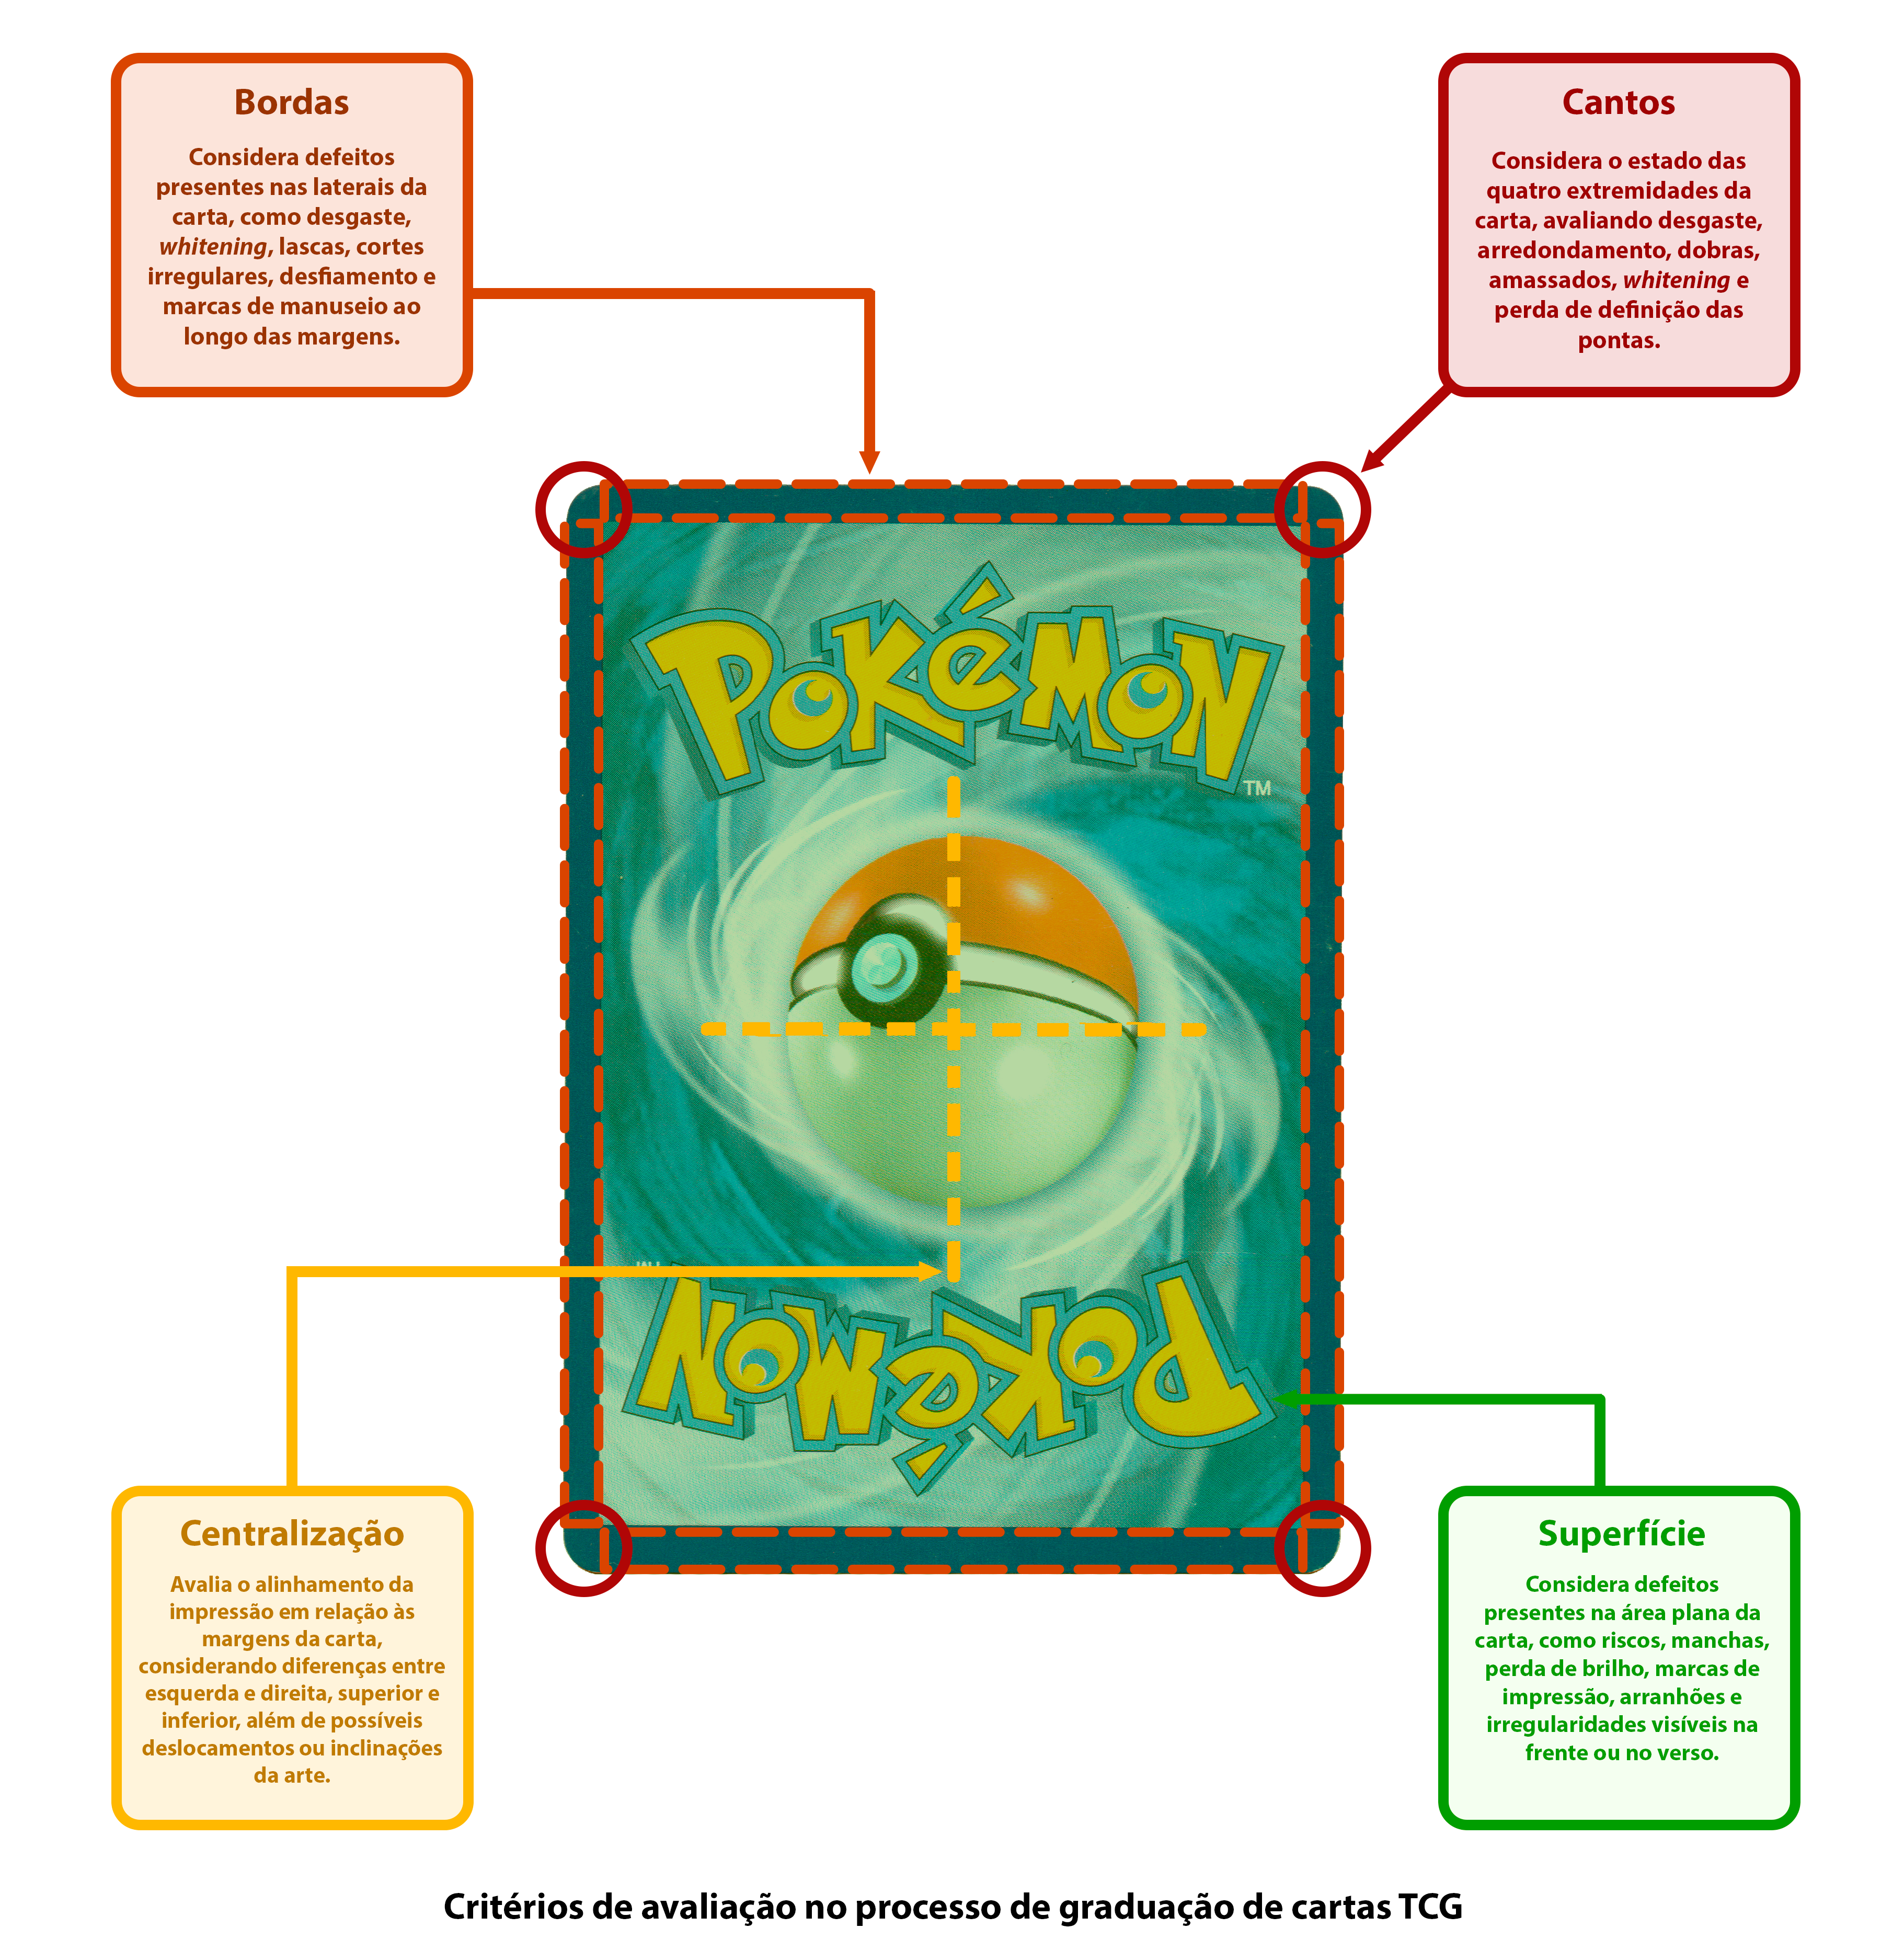
\includegraphics[width=0.78\textwidth]{assets/criterios_1.png}

    
    \legend{Fonte: Elaborado pelo autor a partir de imagem fornecida 
    por empresa parceira (2026).}
\end{figure}

Do ponto de vista computacional, compreender a aparência desses
defeitos é necessário para formular a tarefa de detecção. Os tipos de
defeito observados nas cartas do conjunto de dados deste trabalho
incluem:

\begin{itemize}
    \item \textbf{Riscos (\textit{scratches}):} marcas finas e
    alongadas na superfície, na frente ou no verso da carta, de
    comprimento e visibilidade variáveis.

    \item \textbf{Vincos e dobras (\textit{creases}):} deformações do
    papel resultantes de dobramento parcial, que na fotografia aparecem
    como linhas mais claras ou mais escuras que a superfície ao redor.

    \item \textbf{\textit{Whitening}:} perda de pigmento nas bordas ou
    nos cantos, que ficam mais claros que o restante da carta.

    \item \textbf{Desgaste de cantos (\textit{corner wear}):}
    arredondamento ou amassamento das pontas da carta pelo manuseio.

    \item \textbf{Desgaste de bordas (\textit{edge wear}):}
    irregularidades ao longo das bordas, frequentemente acompanhadas de
    \textit{whitening}.

    \item \textbf{Manchas e pontos:} marcas de sujeira sobre a
    superfície, de poucos pixels a regiões extensas.
\end{itemize}

Ocorre também um desgaste difuso, formado por muitos micro-riscos ou
micro-pontos sem início nem fim definidos, que não pode ser delimitado
por caixas; seu tratamento é descrito no
Capítulo~\ref{cap:desenvolvimento}.

Esses defeitos apresentam
características que dificultam sua detecção automática. Muitos ocupam
regiões pequenas em relação à área da carta, como é comum em defeitos
superficiais \cite{Chen2021}; a análise de tamanho apresentada na
Seção~\ref{sec:contextualizacao} quantifica isso para este conjunto de
dados. Defeitos sutis sobre superfícies com texturas e padrões visuais
complexos representam um desafio reconhecido na literatura de inspeção
visual, o que tem motivado o desenvolvimento de detectores específicos
para esse tipo de cenário \cite{Xia2023}; nas cartas, esse papel é
desempenhado pela arte impressa e pelas superfícies holográficas
(\textit{foil}), cujo reflexo foi discutido na mesma seção. Além disso,
a qualidade da iluminação na captura condiciona o contraste com que o
defeito aparece na imagem \cite{Zheng2021}.

A relevância de um sistema automatizado decorre dessas dificuldades e
do caráter manual da graduação, descrito no
Capítulo~\ref{cap:introducao}: a inspeção é demorada e sujeita à
subjetividade de cada avaliador \cite{Nahar2025}. Neste trabalho, o
detector não atribui nota à carta; ao localizar cada defeito por caixa
delimitadora, ele indica ao avaliador em que pontos concentrar a
inspeção.

\subsection{Detecção de Objetos}
\label{subsec:deteccao_objetos}

A detecção de objetos é uma tarefa de visão computacional que combina 
dois problemas distintos: a classificação de objetos presentes em uma 
imagem e a localização precisa de cada instância por meio de caixas 
delimitadoras (\textit{bounding boxes}) \cite{Hussain2023}. Diferentemente 
da classificação de imagens, que atribui um único rótulo à imagem 
inteira, a detecção de objetos é capaz de identificar múltiplos 
objetos em posições diferentes, retornando para cada um deles 
suas coordenadas espaciais, a classe correspondente e um escore 
de confiança \cite{Ramos2025}.

A qualidade de uma detecção é medida pela métrica
\textit{Intersection over Union} (IoU), que quantifica a sobreposição
entre a caixa delimitadora predita e a caixa de referência
(\textit{ground truth}). O IoU é calculado como a razão entre a área de
interseção e a área de união das duas caixas \cite{Xu2022}, assumindo
valores entre 0 e 1, em que valores mais próximos de 1 indicam maior
precisão de localização. A partir de um limiar de IoU, como o de 0,5,
usado na métrica apresentada na Seção~\ref{subsec:metricas}
\cite{Ramos2025}, uma predição é considerada verdadeiro positivo (TP)
quando corresponde a uma caixa de referência e sua sobreposição atinge
ou supera esse limiar. A correspondência é de um para um: cada caixa
de referência pode ser associada a uma única predição, e predições que
não correspondem a nenhuma caixa de referência, inclusive uma segunda
predição sobre o mesmo defeito, são contabilizadas como falsos positivos
(FP), e caixas de referência que não são associadas a nenhuma predição
válida são contabilizadas como falsos negativos (FN).

As arquiteturas de detecção de objetos são geralmente 
classificadas em dois grupos: detectores de dois estágios 
(\textit{two-stage}) e detectores de um estágio 
(\textit{one-stage}) \cite{Hussain2023}. Os detectores de dois 
estágios, como a família R-CNN, dividem o processo em uma etapa 
de geração de propostas de regiões candidatas e uma etapa 
posterior de classificação e refinamento. Embora apresentem alta 
acurácia, esse design resulta em maior custo computacional e 
menor velocidade de inferência \cite{Situ2023}. Os detectores 
de um estágio, por sua vez, realizam a classificação e a 
localização em uma única passagem pela rede, obtendo melhor 
desempenho em tempo real com menor demanda computacional 
\cite{Hussain2023}.

Como discutido na Seção~\ref{sec:contextualizacao}, a detecção de
objetos é preferida à classificação quando a localização do defeito é
necessária \cite{Hussain2023}. Nas cartas, riscos, desgastes e pequenas
dobras ocupam regiões específicas e reduzidas da superfície, de modo
que a localização de cada defeito é parte central da análise.

% ---------------------------------------------------------------
\subsection{Métricas de Avaliação}
\label{subsec:metricas}

A avaliação de modelos de detecção de objetos requer métricas
que considerem simultaneamente a acurácia de classificação
e a qualidade de localização espacial \cite{Ramos2025}.
As métricas fundamentais são a precisão (\textit{precision})
e a revocação (\textit{recall}), definidas respectivamente
como:

\begin{equation}
    \text{Precisão} = \frac{TP}{TP + FP}
\end{equation}

\begin{equation}
    \text{Revocação} = \frac{TP}{TP + FN}
\end{equation}

em que TP são os verdadeiros positivos, FP os falsos positivos
e FN os falsos negativos. A precisão mede
a proporção de detecções corretas entre todas as detecções
realizadas, enquanto a revocação mede a proporção de objetos
reais que foram corretamente detectados. O F1-\textit{score}
combina ambas as métricas em um único valor por meio da
média harmônica:

\begin{equation}
    F1 = 2 \cdot \frac{\text{Precisão} \times \text{Revocação}}
    {\text{Precisão} + \text{Revocação}}
\end{equation}

Cada caixa predita pelo detector vem acompanhada de um escore de
confiança, como apresentado na Seção~\ref{subsec:deteccao_objetos}.
A precisão, a revocação e o F1 dependem, portanto, de um limiar de
confiança: só as predições com confiança igual ou superior a ele são
contadas. Um limiar baixo aceita mais predições, o que tende a
aumentar a revocação e a reduzir a precisão; um limiar alto produz o
efeito inverso. O F1 pode ser calculado sobre todas as caixas de um
conjunto de avaliação, o F1 agregado, ou separadamente para cada
carta, com as predições e as anotações das suas duas faces, o F1 por
carta. Como todas as cartas do conjunto de dados têm ao menos uma
anotação, o F1 por carta está definido para todas elas, exceto nas
verificações feitas sem as caixas sugeridas, em que cinco cartas ficam
sem nenhuma anotação e saem das comparações por carta
(Seção~\ref{subsec:dados}). A forma como o limiar foi escolhido neste trabalho é descrita
na Seção~\ref{subsec:validacao_cruzada}, e o uso do F1 por carta como
nota das comparações pareadas, na
Seção~\ref{subsec:comparacao_estatistica}.

A métrica de referência na avaliação de detectores de objetos
é o \textit{mean Average Precision} (mAP), que resume o
desempenho do modelo ao calcular a média das precisões médias
(\textit{Average Precision} -- AP) para cada classe
\cite{Ramos2025}. A AP de uma classe é calculada como a área
sob a curva precisão-revocação, que varia conforme o limiar
de confiança das predições. O mAP é então a média das APs
sobre todas as classes:

\begin{equation}
    \text{mAP} = \frac{1}{N} \sum_{i=1}^{N} AP_i
\end{equation}

em que $N$ é o número de classes. Neste trabalho, com a classe
única \textit{defeito}, o mAP coincide com a AP dessa classe. Duas
variantes são frequentemente reportadas na literatura: o mAP@0,5,
que utiliza um limiar de IoU de 0,5 para classificar predições como
TP, e o mAP@0,5:0,95, que calcula a média sobre os limiares de IoU
de 0,5 a 0,95, em passos de 0,05 \cite{Ramos2025}.

% ---------------------------------------------------------------

\subsection{Arquitetura YOLO}
\label{subsec:yolo}

A família YOLO (\textit{You Only Look Once}) representa uma das abordagens
de detecção de objetos do tipo \textit{one-stage} mais difundidas na literatura
recente, destacando-se pelo equilíbrio entre velocidade de inferência e acurácia
\cite{Ramos2025}. Desde sua formulação inicial, a arquitetura trata a detecção
como um problema unificado, prevendo caixas delimitadoras e probabilidades de
classe diretamente a partir da imagem em uma única passagem pela rede
\cite{Hussain2023}. Essa característica diferencia os modelos YOLO de detectores
em duas etapas, nos quais a geração de regiões candidatas e a classificação são
realizadas em fases separadas.

Ao longo do tempo, diferentes versões da família YOLO incorporaram melhorias
voltadas ao tratamento de objetos em múltiplas escalas, à otimização do
treinamento e à eficiência computacional \cite{Hussain2023,Ramos2025}. O YOLOv8,
lançado em 2023, mantém a estrutura modular do YOLOv5, composta por \textit{backbone},
a parte que extrai as características da imagem, \textit{neck}, que
combina essas características em várias escalas, e \textit{head}, a
cabeça que produz as caixas e as classes. De versões anteriores da
família, ele conserva no \textit{neck} a PANet (\textit{Path
Aggregation Network}), estrutura que combina características de
diferentes resoluções, e a cabeça com ramos desacoplados para
classificação e regressão, introduzida em uma versão posterior ao
YOLOv5; em relação ao YOLOv5, entre as novidades estão a
detecção \textit{anchor-free} e um novo bloco de extração de
características no \textit{backbone}, o C2f \cite{Ramos2025}.

Nas versões anteriores, a rede previa deslocamentos em relação a caixas
de formatos predefinidos, chamadas caixas âncora, distribuídas sobre o
mapa de características. O paradigma \textit{anchor-free} dispensa essas
caixas: o modelo prevê diretamente os centros dos objetos.
Essa característica simplifica o treinamento e pode favorecer a adaptação a
conjuntos de dados específicos, nos quais as proporções e distribuições dos objetos
não seguem necessariamente os padrões de bases genéricas \cite{Ramos2025}. Já o
módulo C2f busca melhorar o reaproveitamento de características intermediárias,
aumentando a capacidade de representação do \textit{backbone} sem comprometer a
eficiência computacional. A PANet, por sua vez, contribui para a fusão
de informações em diferentes resoluções \cite{Ramos2025}, como detalhado
a seguir.

Como apresentado na Seção~\ref{sec:contextualizacao}, a rede reduz a
imagem de entrada em etapas, e cada ponto de um mapa de características
resume um bloco de pixels da imagem cujo lado é o passo. No YOLOv8, o
\textit{backbone} realiza cinco dessas etapas, cada uma dividindo pela
metade a largura e a altura do mapa. Os mapas obtidos formam níveis,
identificados pela letra P seguida do número da etapa: no nível P$k$,
cada ponto resume um bloco de $2^k \times 2^k$ pixels, de modo que o
passo vale 2 pixels no nível P1, 4 no P2, 8 no P3, 16 no P4 e 32 no P5
\cite{Jocher2023}. Quanto mais alto o nível, maior a região da imagem
resumida por cada ponto e menor o detalhe espacial que o mapa preserva.
A Figura~\ref{fig:niveis_p} mostra os blocos dos níveis P2 a P5 sobre
um defeito do conjunto de dados deste trabalho, na resolução de entrada
de 640 pixels: com menor lado de 6,9 pixels, o defeito é menor que um
único bloco do nível P3. O \textit{neck} mistura a informação desses
níveis nos dois sentidos. No caminho de cima para baixo, de desenho
inspirado na rede de pirâmide de características (FPN, do inglês
\textit{Feature Pyramid Network}), os mapas mais reduzidos são ampliados
e combinados aos mais detalhados; a PANet, citada acima, acrescenta um
caminho de baixo para cima, que complementa o primeiro e leva o detalhe
espacial dos mapas mais detalhados até os mais reduzidos
\cite{Ramos2025}. Na configuração padrão do YOLOv8, a cabeça de detecção
decide sobre três níveis: P3, destinado aos objetos pequenos, P4, aos
médios, e P5, aos grandes \cite{Jocher2023}. Os níveis P1 e P2 existem
no \textit{backbone}, mas não recebem cabeça de detecção; por isso, o
menor passo sobre o qual o modelo padrão decide é de 8 pixels. A
biblioteca oferece também uma variante, chamada P2, que acrescenta uma
cabeça de detecção sobre o nível P2, de passo 4; ela é
descrita na Seção~\ref{subsec:objetos_pequenos}.

\begin{figure}[H]
    \centering
    \caption{Blocos resumidos por um ponto nos níveis P2 a P5, sobre um
    defeito do conjunto de dados, na imagem de entrada de 640 pixels.}
    \label{fig:niveis_p}
    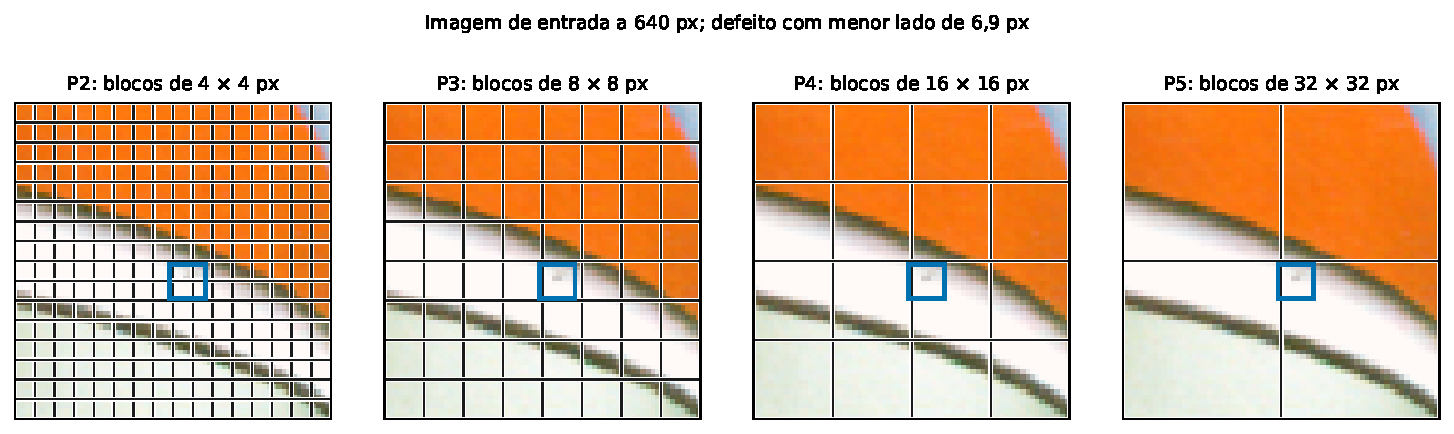
\includegraphics[width=\textwidth]{assets/figuras/206/figE2_niveis_p.pdf}
    \legend{Fonte: Elaborado pelo autor (2026).}
\end{figure}

Os pesos pré-treinados do YOLOv8 disponibilizados pela Ultralytics foram
obtidos no conjunto COCO (\textit{Common Objects in Context}), uma base de
imagens de objetos comuns em cenas do cotidiano \cite{Lin2014}, em sua
versão de 2017, cujo conjunto de treino reúne cerca de 118 mil imagens
anotadas em 80 classes \cite{Jocher2023}. Esses pesos constituem o ponto
de partida usual para adaptar o YOLOv8 a novos domínios, seja por
inferência direta, seja por ajuste fino (\textit{fine-tuning}), descrito
na Seção~\ref{subsec:transfer_learning} \cite{Dobrzycki2025, Situ2023}.

No presente trabalho, a escolha do YOLOv8 está relacionada à sua 
adequação ao problema investigado. Como os defeitos em cartas
podem ser pequenos, localizados e visualmente sutis, a tarefa exige
um detector capaz de preservar informações espaciais e operar de
forma eficiente. Em comparação com detectores de dois estágios, como
a família R-CNN, detectores de um estágio como o YOLO oferecem menor
custo computacional e maior velocidade de inferência
\cite{Situ2023, Hussain2023}, embora com acurácia em geral inferior
\cite{Hussain2023}; o menor custo viabilizou treinar as várias
configurações comparadas no equipamento disponível. Além disso, o
YOLOv8 possui variantes com diferentes relações entre custo
computacional e desempenho \cite{Ramos2025}. Em cenários de
adaptação de modelos pré-treinados, \citeonline{Dobrzycki2025} 
investigam estratégias de \textit{transfer learning} em arquiteturas 
YOLOv8 e YOLOv10, demonstrando que a escolha da configuração de 
treinamento depende das características do conjunto de dados e dos 
recursos computacionais disponíveis.

O modelo de partida (\textit{baseline}) adotado neste trabalho foi o
YOLOv8s inicializado com pesos pré-treinados no COCO e submetido a
ajuste fino sobre as imagens de cartas Pokémon TCG, com a classe única
\textit{defeito}. Treinado com imagens RGB e sem aumento de dados, esse
modelo corresponde à Configuração 1 e serviu de referência para o
estudo fatorial, que mediu o efeito do aumento de dados e do realce de
micro-relevo. A cabeça de detecção adicional P2 e a resolução de
entrada foram avaliadas depois, alterando-se um componente por vez
sobre a configuração de melhor desempenho, procedimento apresentado na
Seção~\ref{subsec:ablacao_conceito} e detalhado no
Capítulo~\ref{cap:desenvolvimento}.

% ---------------------------------------------------------------
\subsection{Transfer Learning}
\label{subsec:transfer_learning}

\textit{Transfer learning} é uma estratégia de aprendizado de
máquina que consiste em aproveitar o conhecimento adquirido por
um modelo treinado em um domínio fonte para melhorar o
desempenho em um domínio alvo distinto \cite{Situ2023}.
A motivação para essa abordagem reside na observação de que
modelos profundos aprendem representações hierárquicas de
características visuais que tendem a ser transferíveis entre
domínios, especialmente nas camadas mais rasas da rede, que
capturam padrões genéricos como bordas, texturas e gradientes
\cite{Situ2023}.

Na prática, o \textit{transfer learning} em visão computacional
é implementado por meio do ajuste fino: um modelo pré-treinado em
um conjunto de dados de larga escala, como ImageNet ou COCO, tem
seus pesos utilizados como ponto de partida, sendo então re-treinado
total ou parcialmente sobre o conjunto de dados alvo
\cite{Dobrzycki2025}. Essa abordagem permite que o modelo se
adapte às características específicas do novo domínio sem
partir de uma inicialização aleatória, reduzindo
significativamente a quantidade de dados rotulados necessária
para alcançar bom desempenho \cite{Situ2023}.

Em cenários com baixo volume de dados, o \textit{transfer learning} é
especialmente relevante. Um modelo treinado do zero com poucas imagens
tende ao sobreajuste (\textit{overfitting}): ele se ajusta aos exemplos
de treino, inclusive aos detalhes particulares de cada um, e passa a
errar em imagens novas. \citeonline{He2019} mediram esse efeito em
detecção de objetos. Com apenas mil imagens de treino do COCO, um
detector de dois estágios que partiu de pesos pré-treinados no ImageNet
atingiu 9,9 pontos de AP, em uma escala de 0 a 100. O mesmo detector
treinado do zero atingiu 3,5, e os autores atribuem essa diferença ao
sobreajuste causado pela falta de dados. Quando o número de imagens de
treino aumentou, a vantagem do pré-treino diminuiu. Isso indica que o
pré-treino ajuda mais justamente quando há poucos dados.

Esse benefício, porém, vale apenas para as camadas que já existiam no
modelo pré-treinado. Quando uma parte nova é acrescentada à
arquitetura, como um nível de detecção a mais, essa parte e as camadas
que mudam de posição ou de formato para recebê-la, como a própria cabeça de
detecção, não têm pesos pré-treinados correspondentes e começam com
valores aleatórios, situação verificada na variante usada neste trabalho
e quantificada no Capítulo~\ref{cap:desenvolvimento}. \citeonline{LiM2023}
mediram o efeito de manter partes de um detector com valores
aleatórios. Quando o \textit{neck} e a cabeça de detecção também
receberam pré-treino, o desempenho foi maior do que quando começaram
aleatórios, inclusive quando o ajuste fino usou apenas 1\% das imagens
de treino do COCO. Para os autores, começar com partes aleatórias é uma
das diferenças entre o pré-treino e o ajuste fino que podem limitar o
resultado e tornar a convergência mais lenta. Esses detectores não eram
da família YOLO, e o estudo não tratou de camadas acrescentadas a um
modelo existente; por isso, neste trabalho, essa relação é tratada como
hipótese para explicar o desempenho da variante com a cabeça P2,
descrita na Seção~\ref{subsec:objetos_pequenos}, e é examinada com os
resultados no Capítulo~\ref{cap:desenvolvimento}.

% ---------------------------------------------------------------
\subsection{Detecção de Objetos em Cenários com Dados Limitados}
\label{subsec:low_data_detection}

A detecção de objetos em cenários com dados limitados constitui um
problema relevante em visão computacional, especialmente em domínios
nos quais a coleta e a anotação de imagens são custosas. Neste trabalho,
o termo \textit{baixo volume de dados} refere-se a conjuntos nos quais
o número de exemplos anotados é insuficiente para treinar modelos de
detecção profundos com capacidade de generalização adequada, tornando
necessário o uso de estratégias complementares como \textit{transfer
learning} e aumento de dados \cite{Chen2021}. Não há um limiar absoluto
para esse conceito, pois o volume que se mostra limitado depende da
tarefa e do modelo. No presente trabalho, esse cenário é caracterizado
pelo conjunto de 206 cartas disponível, volume inferior ao das 593
cartas esportivas usadas por \citeonline{Nahar2025} na classificação de
cantos, conjunto que os próprios autores caracterizam como pequeno.

Em tarefas de detecção, além de reconhecer a classe de interesse,
o modelo também deve localizar espacialmente cada instância na imagem
por meio de caixas delimitadoras \cite{Ramos2025}. Essa exigência torna
o processo mais sensível à escassez de exemplos rotulados, uma vez que,
além da imagem, é necessário dispor de anotações consistentes indicando
a localização de cada objeto ou defeito de interesse \cite{Situ2023}.
Em conjuntos reduzidos, modelos baseados em \textit{deep learning}
tendem a apresentar maior risco de sobreajuste e menor
capacidade de generalização, pois há poucos exemplos disponíveis para
representar adequadamente a variabilidade visual dos objetos ou
defeitos \cite{Wang2022}. Esse problema torna-se ainda mais crítico em
aplicações de inspeção visual, nas quais os defeitos podem ser pequenos,
sutis, desbalanceados e difíceis de distinguir do fundo da imagem
\cite{Chen2021, Wang2022}. A pesquisa não adota um protocolo formal de
\textit{Few-Shot Object Detection}, em que o modelo aprende classes
novas a partir de poucos exemplos em divisões padronizadas dos dados,
porque aqui não há classes novas: o detector aprende uma única classe,
\textit{defeito}, com todas as anotações disponíveis. Ela se insere no
contexto da detecção de objetos com
baixo volume de dados \cite{Situ2023}, avaliando estratégias como
\textit{transfer learning}, aumento de dados e uso de imagens de realce
de micro-relevo para melhorar o desempenho do detector. A cabeça de detecção adicional P2 e a resolução de
entrada, também avaliadas, respondem a outra limitação, o tamanho
reduzido dos defeitos na imagem, tratada na
Seção~\ref{subsec:objetos_pequenos}.

Uma forma de verificar se o volume de dados limita o desempenho é a
curva de aprendizado, que descreve o desempenho de um modelo em função
do tamanho do conjunto de treino \cite{Viering2023}. Ela é obtida
treinando o mesmo modelo com frações crescentes dos dados de treino e
avaliando todas as versões no mesmo conjunto de avaliação. A curva de
aprendizado não se confunde com a curva de treino, que acompanha o
desempenho ao longo de um único treinamento, a cada passagem completa
pelos dados de treino, chamada época. Se o desempenho continua a subir
nas últimas frações, mais dados tendem a melhorar o modelo; se a
inclinação da curva se torna pequena, ela se aproxima de um patamar, e
coletar mais dados rende pouco \cite{Viering2023}. A mesma ferramenta
foi proposta para avaliar decisões de projeto, como o pré-treino e o
aumento de dados, no regime de poucos dados \cite{Hoiem2021}. Estimar
quantos exemplos a mais seriam necessários para atingir um
desempenho-alvo, por outro lado, é mais difícil: extrapolar a curva a
partir de poucos dados produz estimativas pouco confiáveis
\cite{Mahmood2022}. Por isso, neste trabalho, a curva de aprendizado
foi usada para verificar se o desempenho já havia se estabilizado, e
não para prever o número de cartas necessário.

% ---------------------------------------------------------------
\subsection{Aumento de Dados}
\label{subsec:data_augmentation}

O aumento de dados (\textit{data augmentation}) é um conjunto
de técnicas que amplia a diversidade do conjunto de treinamento
por meio de transformações aplicadas às imagens existentes, sem
a necessidade de coletar novos exemplos. O princípio é expor o
modelo, durante o treinamento, a variações plausíveis das
imagens, de modo que ele não dependa de detalhes particulares
dos poucos exemplos disponíveis. Na detecção de defeitos
superficiais com pequenas amostras, o aumento de dados é
apontado como uma das quatro linhas de solução para o problema
\cite{Chen2021}.

As transformações usadas no aumento de dados costumam ser de
dois tipos. As geométricas, como espelhamento, rotação,
translação e mudança de escala, alteram a posição, a orientação
e o tamanho dos objetos na imagem. As fotométricas alteram a cor
e o brilho, por exemplo por variações de matiz, saturação e
valor no espaço de cor HSV (\textit{Hue, Saturation, Value}).
Na biblioteca Ultralytics, usada neste trabalho, essas
transformações são aplicadas durante o treinamento, a cada vez
que uma imagem é carregada, com intensidade sorteada dentro de
limites definidos nos parâmetros de configuração do treino,
chamados hiperparâmetros \cite{Jocher2023}. A biblioteca oferece
também o mosaico, que combina quatro imagens de treino em uma
única imagem e recorta dela uma janela do tamanho da entrada da
rede. A mudança de escala, por sua vez, amplia
ou reduz a imagem por um fator sorteado; quando reduz, os
objetos ficam menores, o que importa quando eles já estão
próximos do passo do nível de detecção mais fino, apresentado
na Seção~\ref{subsec:yolo}.

Em cenários com conjuntos de dados reduzidos, o aumento de
dados atua contra o sobreajuste: ao aumentar a diversidade
efetiva do conjunto de treinamento, reduz a dependência do
modelo em relação a padrões específicos dos exemplos
disponíveis \cite{Chen2021}. Uma medição do tamanho desse
efeito vem da classificação de imagens: com ajuste fino, o erro
obtido com aumento de dados foi aproximadamente igual ao obtido
sem ele usando 1,8 vez mais exemplos, o que levou os autores a
interpretar o aumento de dados como um multiplicador do valor
de cada exemplo \cite{Hoiem2021}. Neste trabalho, o aumento de
dados foi um dos dois fatores do estudo fatorial, o que
permitiu medir seu efeito isolado e combinado com o realce de
micro-relevo.

% ---------------------------------------------------------------
\subsection{Pré-processamento e realce de micro-relevo}
\label{subsec:fotometria}

Em uma fotografia, o relevo da superfície não é registrado
diretamente: ele aparece apenas de forma indireta, como variações
locais de brilho, porque a inclinação do papel em um vinco ou em
um amassado altera a quantidade de luz refletida em direção à câmera.
A intensidade dessas variações depende da iluminação da captura, que
condiciona o contraste com que o defeito aparece na imagem
\cite{Zheng2021}. O realce de micro-relevo não reconstrói a forma
tridimensional da superfície; ele amplifica essas variações locais de
brilho, para que se destaquem do restante da imagem. Métodos
baseados em filtragem, como transformada de Fourier, filtros de Gabor
e transformada \textit{wavelet}, integram o repertório clássico de
detecção de defeitos em superfícies \cite{Chen2021}, e operadores de
filtragem também têm sido aplicados como etapa de pré-processamento
em sistemas de inspeção visual \cite{Sawada2024, Jiang2023}.

No contexto da inspeção visual automatizada, filtros de gradiente
direcional têm sido aplicados como etapa de pré-processamento para
realce de defeitos em superfícies industriais. \citeonline{Sawada2024}
empregam o filtro \textit{emboss}, que realça a variação de intensidade
em uma direção e dá à imagem aparência de relevo, aplicado em oito
direções, na etapa de extração
de defeitos em superfícies pintadas, dentro de um pipeline clássico de
morfologia matemática que antecede a classificação por rede
convolucional. Os autores não avaliam isoladamente a contribuição do
realce por gradiente, de modo que o trabalho evidencia a aplicabilidade
da técnica ao problema, e não sua superioridade sobre a ausência de
pré-processamento. De forma complementar,
\citeonline{Jiang2023} combinam a equalização adaptativa de histograma
com limitação de contraste (CLAHE, do inglês \textit{Contrast Limited
Adaptive Histogram Equalization}) a um método de equalização automática
de cor (ACE), fundindo as duas imagens realçadas, como
pré-processamento anterior à detecção com o YOLOv3. Como o CLAHE não
foi avaliado separadamente, o trabalho mostra que o operador já foi
empregado antes de um detector da família YOLO, e não o seu efeito
isolado; na representação adotada neste trabalho, ele foi aplicado
apenas ao brilho da imagem,
como um dos canais da representação de entrada descrita adiante.
Os operadores de gradiente direcional respondem à
taxa de variação da intensidade, isto é, a bordas. Defeitos como riscos
e vincos, contudo, não constituem bordas, e sim estruturas alongadas de
espessura reduzida com intensidade semelhante nos dois lados, que
correspondem a estruturas de segunda ordem. \citeonline{Gruber2021}
sustentam que a filtragem baseada nos autovalores da matriz Hessiana, que
descreve a curvatura local da intensidade da imagem, é adequada à inspeção de superfícies precisamente porque os defeitos
observados são acompanhados de estruturas dessa natureza, e registram
que as derivadas que compõem a Hessiana são obtidas pela convolução da
imagem com as derivadas de uma função gaussiana, chamada núcleo, cujo
desvio padrão determina a escala das estruturas amplificadas. Essa seletividade de escala é relevante no
presente caso, uma vez que a carta apresenta arte impressa cujos
contornos possuem escala e contraste superiores aos dos defeitos
investigados, e que operadores de primeira ordem amplificam de forma
indistinta.

A representação de realce adotada neste trabalho ocupa os três canais
de entrada com a luminosidade original da imagem, com essa luminosidade
realçada por um primeiro operador e com a resposta de um segundo
operador, calculada sobre a imagem já realçada. O primeiro
é o CLAHE. Nele, a imagem é dividida em uma grade de regiões
retangulares, chamadas ladrilhos; o histograma de intensidades de cada
ladrilho é equalizado, o que estica o contraste dentro dele; um limite
de corte restringe esse estiramento, para não amplificar o ruído; e os
resultados de ladrilhos vizinhos são combinados por interpolação
bilinear \cite{Jiang2023}. Neste trabalho, o CLAHE foi aplicado ao
canal de luminosidade (L$^*$) do espaço de cor CIELAB, que separa o brilho
da cor, e não aos três canais RGB; assim, ele atua sobre o brilho, em
que o relevo se manifesta, sem alterar a cor. O segundo operador é a
medida de \citeonline{Frangi1998}, calculada a partir dos autovalores
da matriz Hessiana em várias escalas: ela responde a estruturas
alongadas, como cristas e vales, e atenua regiões uniformes e manchas
arredondadas. Os autores fixaram em 0,5 o parâmetro que controla a
sensibilidade ao alongamento da estrutura e indicaram, para o
parâmetro que controla a supressão das regiões de baixo contraste,
metade do maior valor da norma da Hessiana na imagem, valor que
funcionou na maioria dos casos que avaliaram. Esses mesmos valores foram
usados neste trabalho. Por construção, a medida favorece os defeitos
alongados, como riscos e vincos, e tende a atenuar manchas, pontos e o
\textit{whitening} em área, que também estão entre os defeitos do
conjunto de dados; a luminosidade original e a luminosidade com CLAHE, nos
outros dois canais, preservam a informação desses defeitos.

O YOLOv8 pré-treinado espera uma imagem de três canais.
\citeonline{JiangJ2021} observam que, quando a entrada tem um único
canal, a solução mais simples é replicá-lo três vezes, o que
desperdiça dois canais. Na detecção de navios em imagens de radar, que
têm um único canal, os autores substituíram duas das cópias por
versões da mesma imagem que destacam os detalhes finos (sub-bandas de
alta frequência), e o AP do YOLO-V4-tiny passou de 88,08\% para
89,64\%, um ganho de 1,56 ponto percentual. Na mesma linha, a
representação de realce de micro-relevo avaliada neste trabalho ocupa
os três canais com informações diferentes da mesma imagem; sua
composição e o procedimento que a escolheu entre as alternativas
testadas são descritos na Seção~\ref{subsec:estrategias}. Essa
substituição tem um custo possível: as primeiras camadas da rede
pré-treinada aprenderam padrões de imagens RGB comuns, e uma entrada
formada por canais realçados se afasta dessa distribuição, o que pode
reduzir parte do benefício do pré-treino descrito na
Seção~\ref{subsec:transfer_learning}. \citeonline{Ahmad2025} observaram
uma tendência compatível com essa hipótese ao aplicar o CLAHE a
radiografias de coluna, na segmentação de vértebras com um Mask R-CNN:
o modelo pré-treinado teve uma pequena queda na sobreposição entre a
segmentação prevista e a real, e o mesmo modelo treinado do zero, um
ganho marginal. Nenhuma das duas diferenças foi estatisticamente
significativa. Os autores sugerem que o realce introduz uma mudança de
domínio que pode reduzir a utilidade das características
pré-treinadas. No trabalho de \citeonline{JiangJ2021}, a entrada
original já tinha um único canal, situação diferente da substituição de
uma imagem RGB. Até onde
a busca bibliográfica identificou, o uso de uma representação de
realce de micro-relevo como entrada de um detector YOLOv8 não havia
sido investigado na inspeção de cartas colecionáveis.

\subsection{Detecção de objetos pequenos}
\label{subsec:objetos_pequenos}

A detecção de objetos pequenos constitui um subcampo com dificuldades
próprias, distintas das que caracterizam a detecção em cenários com dados
limitados. \citeonline{Cheng2023} identificam a perda de informação como um
de seus desafios centrais: detectores convencionais reduzem progressivamente
a resolução espacial ao longo do \textit{backbone}, e a decisão da cabeça de
detecção é tomada sobre a representação resultante. Essa perda praticamente
não afeta objetos grandes e médios, cujas características sobrevivem à
subamostragem, mas é determinante para objetos pequenos, dos quais resta
pouca informação nas camadas finais.

Essa perda está ligada ao passo dos níveis de detecção, apresentado na
Seção~\ref{subsec:yolo}. Na resolução de entrada de 640 pixels, o nível
P3, de passo 8, é um mapa de até $80 \times 80$ pontos, cada qual
resumindo um bloco de $8 \times 8$ pixels da imagem de entrada. Um
defeito cujo menor lado é menor que 8 pixels ocupa apenas parte de cada
bloco em que aparece; o restante do bloco é fundo, isto é, a superfície
da carta ao redor do defeito. O ponto que resume o bloco combina os dois
sinais, e o do defeito fica diluído no do fundo: enfraquecido, mas não
necessariamente ausente. Por isso, a detecção desses defeitos é mais
difícil, sem ser impossível. Em defeitos de placas de circuito impresso,
\citeonline{Xia2023} afirmam que as características de alvos menores que
$10 \times 10$ pixels se tornam muito fracas, ou desaparecem por
completo, no mapa de passo 8.

Há duas formas diretas de reduzir essa limitação. A primeira é
acrescentar um nível de detecção mais fino. Na variante P2 do YOLOv8, a
cabeça de detecção passa a decidir também sobre o nível P2, de passo 4,
além de P3, P4 e P5, e o \textit{neck} ganha as camadas necessárias para
levar as características até esse nível \cite{Jocher2023}. Como o mapa
de passo 4 tem quatro vezes mais pontos que o de passo 8, o custo de
memória e de processamento aumenta; em um YOLOv8l, o acréscimo do nível
P2 elevou o custo computacional em cerca de 20\% \cite{Liu2026}. Há
também um efeito colateral apontado na literatura. Em defeitos de placas
de circuito impresso, com um YOLOv5s, o acréscimo do nível P2 manteve o
mAP@0,5 em 97,7\%, elevou o mAP@0,5:0,95 de 68,4\% para 73,3\% e a
revocação de 95,5\% para 96,5\%, enquanto a precisão passou de 98,8\%
para 98,1\%; os autores apontam que o mapa P2 traz ruído de fundo e o
tratam com um módulo de atenção ao contexto global \cite{Xia2023}.

A segunda forma é aumentar a resolução de entrada. Como a imagem é
redimensionada até que seu lado maior meça a resolução de entrada,
conforme descrito na Seção~\ref{sec:contextualizacao}, dobrar essa
resolução dobra o tamanho, em pixels, de cada defeito, e o detalhe
ganho é real quando a fotografia original tem mais pixels do que a
resolução de entrada, como ocorre neste conjunto de dados. A
Figura~\ref{fig:resolucao} mostra o mesmo defeito da
Figura~\ref{fig:niveis_p} nas duas resoluções: o menor lado passa de 6,9
para 13,8 pixels, e o defeito, antes menor que um bloco do nível P3,
passa a ser maior que ele. \citeonline{Liu2026} compararam as duas formas
na detecção de objetos pequenos em imagens de drone, com o YOLOv8l:
passar a resolução de entrada de 640 para 1280 pixels elevou o mAP@0,5
de 12,7\% para 15,9\%, um ganho relativo de 25\%, ao custo de cerca de
quatro vezes mais processamento, enquanto o acréscimo do nível P2,
medido a 640 pixels, elevou-o de 12,7\% para 13,5\%, um ganho relativo
de 6\%. Os lotes de treinamento, isto é, o número de imagens processadas
a cada atualização dos pesos, foram diferentes nas duas resoluções (8
imagens a 640 pixels e 4 a 1280), o que limita a comparação direta.
Neste trabalho, a cabeça P2 foi avaliada na resolução de 1280 pixels,
condição que os autores não mediram.

\begin{figure}[H]
    \centering
    \caption{O mesmo defeito na imagem de entrada de 640 e de 1280 pixels,
    com a grade de 8 pixels do nível P3 sobre a mesma região da carta.}
    \label{fig:resolucao}
    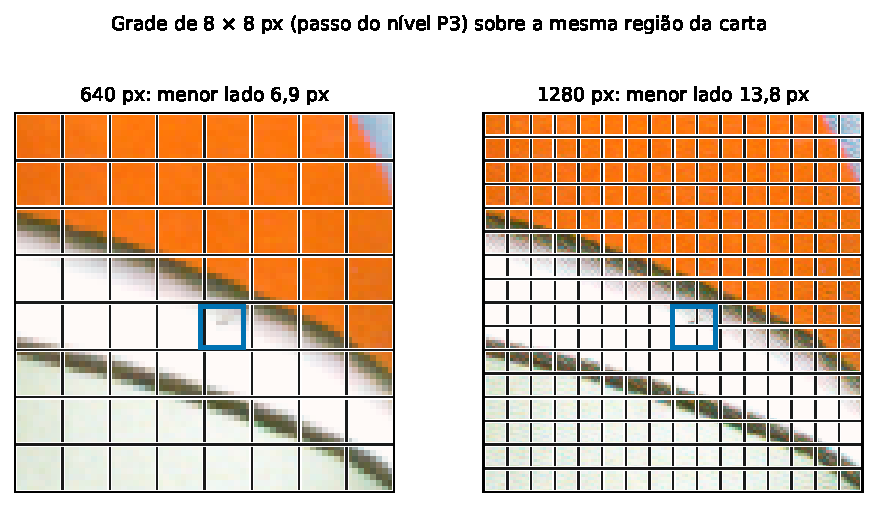
\includegraphics[width=0.75\textwidth]{assets/figuras/206/figE3_resolucao.pdf}
    \legend{Fonte: Elaborado pelo autor (2026).}
\end{figure}

A dificuldade não se restringe à arquitetura: alcança também a métrica de
avaliação. \citeonline{Xu2022} demonstram que a \textit{Intersection over
Union} é altamente sensível ao desvio de localização quando o objeto é
diminuto. Para um objeto de $5 \times 8$ pixels, aumentar o desvio da
caixa predita de 1 para 3 pixels, na diagonal, reduz o IoU de 0,54 para
0,14; para um objeto de $200 \times 320$ pixels, o mesmo aumento o reduz
apenas de 0,97 para 0,91. Em termos práticos, quanto menor o objeto, menor
a tolerância a erro de localização admitida pela métrica. Como a própria
caixa de referência é traçada à mão e sua borda pode variar em alguns
pixels, parte dos defeitos pequenos pode não atingir o limiar de IoU mesmo
com uma predição bem localizada, o que limita o desempenho mensurável
nesses defeitos independentemente da capacidade do detector de percebê-los.

\subsection{Estudo fatorial e estudo de ablação}
\label{subsec:ablacao_conceito}

O estudo de ablação é uma estratégia experimental utilizada para
avaliar a contribuição de componentes específicos de um modelo
ou \textit{pipeline}. Em redes neurais profundas, esse tipo de estudo
consiste em medir o desempenho do modelo após a remoção ou alteração
de determinados componentes, permitindo compreender a contribuição
relativa desses elementos para o desempenho geral \cite{Sheikholeslami2021}.
Em vez de analisar apenas o desempenho de uma configuração final completa,
a ablação compara diferentes versões do experimento, adicionando, removendo
ou modificando elementos de forma controlada. Dessa forma, torna-se possível
identificar quais componentes efetivamente contribuem para a melhoria do
desempenho e quais apresentam impacto reduzido ou dependente do contexto.

Em modelos de detecção de objetos baseados em YOLO, esse tipo
de análise é especialmente relevante para avaliar estratégias
de treinamento e adaptação de modelos pré-treinados.
\citeonline{Liu2022} conduziram um estudo de ablação explícito
em uma arquitetura YOLOv5 modificada para detecção de objetos
pequenos em imagens de drone com dados limitados, avaliando a
contribuição individual de cada componente proposto.
\citeonline{Dobrzycki2025} investigaram sistematicamente
diferentes configurações de \textit{transfer learning} em
arquiteturas YOLOv8 e YOLOv10, comparando treinamento do zero,
ajuste fino completo e congelamento parcial de camadas, em que
parte dos pesos é mantida fixa durante o treino, e concluíram
que não há estratégia universalmente superior e que o
desempenho depende das características do conjunto de dados.
\citeonline{Chen2024NHD} também conduziram um estudo de ablação
sobre os componentes propostos para o detector, acrescentando-os
um a um.

O estudo fatorial, por sua vez, cruza todas as opções de dois ou
mais fatores: cada opção de um fator é combinada com cada opção
dos demais, e cada combinação forma uma configuração. Neste
trabalho, os fatores foram o aumento de dados (sem ou com) e a
representação de entrada (RGB ou realce de micro-relevo), o que
resultou em um estudo fatorial $2 \times 2$, com quatro
configurações. Esse desenho contém as comparações de uma
ablação, pois cada estratégia aparece desligada e ligada
enquanto a outra é mantida fixa (com uma ressalva sobre o aumento de
dados, descrita na Seção~\ref{subsec:estrategias}), e por isso também pode ser
descrito como uma ablação. Além dessas comparações, ele permite
verificar se o efeito de um fator depende da opção adotada no
outro, o que alterar um componente por vez não mostra. Essa
dependência é chamada de interação; neste trabalho, ela foi testada
carta a carta, comparando o efeito do aumento de dados com imagens RGB
e com imagens de realce. Ao longo do
texto, a expressão estudo fatorial designa esse cruzamento
$2 \times 2$, e a expressão ablação designa as avaliações feitas
depois dele sobre a configuração de melhor desempenho, em que um
único componente foi alterado por vez: o acréscimo da cabeça de
detecção P2 e a resolução de entrada. Em todas as configurações,
o ajuste fino foi aplicado sem congelamento de camadas.

% ---------------------------------------------------------------
\subsection{Validação Cruzada}
\label{subsec:validacao_cruzada}

A validação cruzada é um método de estimação de desempenho que busca
reduzir a dependência dos resultados em relação a um particionamento
específico dos dados. Na variante em $k$ dobras
(\textit{k-fold cross-validation}), o conjunto de dados é dividido em
$k$ subconjuntos de tamanho aproximadamente igual, chamados dobras. Em
cada uma das $k$ rodadas, uma dobra distinta é reservada para
avaliação, e as demais são usadas para treinamento, de modo que cada
exemplo é avaliado exatamente uma vez, por um modelo que não o viu no
treinamento. Na variante estratificada, a divisão preserva em cada
dobra a proporção das classes \cite{Kohavi1995}; neste trabalho, com
classe única, a estratificação usou outra característica das cartas,
descrita no Capítulo~\ref{cap:desenvolvimento}. Quando o objetivo
não é apenas estimar o desempenho de um modelo, mas comparar
configurações entre si, a média das métricas sobre as rodadas
descarta uma informação útil: todas as configurações foram avaliadas
sobre exatamente as mesmas dobras, o que permite compará-las em
pares, como descrito na Seção~\ref{subsec:comparacao_estatistica}.

Em cenários com baixo volume de dados, essa abordagem é especialmente
relevante: com poucos exemplos, um único particionamento pode
produzir resultados otimistas ou pessimistas, dependendo de quais
amostras caem no conjunto de avaliação \cite{Kohavi1995}. O valor de
$k$ adotado, as dobras mantidas fixas entre todas as configurações e
a forma como as cartas foram distribuídas entre elas são descritos no
Capítulo~\ref{cap:desenvolvimento}.

Em cada rodada, o bloco de treinamento foi subdividido em um conjunto
de treino efetivo e um conjunto de validação interna, com cerca de
20\% das cartas do bloco. A validação interna não participou da
atualização dos pesos, mas foi usada para todas as escolhas feitas
dentro de cada rodada: a parada antecipada
(\textit{early stopping}), que interrompe o treino quando o
desempenho na validação interna deixa de melhorar e mantém os pesos
da melhor época, porque a piora nessa validação sinaliza o início do
sobreajuste \cite{Prechelt1998}; e o limiar de confiança usado no cálculo do F1,
apresentado na Seção~\ref{subsec:metricas}, escolhido como o que
maximizou o F1 nela. Fazer essas escolhas na dobra de avaliação tornaria
a estimativa otimista, porque o erro medido no conjunto usado para
escolher foi diretamente minimizado por essa escolha e não deve ser
usado para estimar o desempenho \cite{Cawley2010}. Por isso, nessas
escolhas, a dobra de avaliação permaneceu isolada durante o
treinamento de cada rodada e foi usada apenas para medir o desempenho
final dessa rodada. O operador de realce de micro-relevo, por sua vez,
foi escolhido uma única vez, na validação interna da rodada da
primeira dobra, e mantido nas demais; como essa validação interna
contém cartas que são avaliadas nas outras rodadas, essa escolha não
ficou isolada delas, limitação discutida no
Capítulo~\ref{cap:desenvolvimento}.

% ---------------------------------------------------------------
\subsection{Comparação estatística entre configurações}
\label{subsec:comparacao_estatistica}

Reportar a média e o desvio padrão de uma métrica sobre as rodadas da
validação cruzada descreve o desempenho de uma configuração, mas não é
suficiente para afirmar que uma configuração supera outra. A variação
decorrente da amostra de avaliação e do próprio treinamento pode ser da
mesma ordem de grandeza que as diferenças entre as configurações
comparadas; por isso, decidir se uma supera a outra exige levar essa
variação em conta, e não apenas comparar médias \cite{Bouthillier2021}.

A alternativa é o teste pareado. Quando as mesmas partições são utilizadas
em todas as configurações, cada unidade de avaliação é observada uma vez em
cada configuração, e a comparação pode ser feita sobre a diferença dentro de
cada par. Com isso, a variação entre as unidades, que é comum às
configurações comparadas, deixa de pesar na incerteza da diferença;
\citeonline{Demsar2006} descreve esse efeito na comparação de dois
classificadores sobre vários conjuntos de dados. Neste trabalho, a unidade
de avaliação foi a carta: com as dobras fixas entre as configurações, cada
uma das 206 cartas foi avaliada uma vez por configuração, por um modelo que
não a viu no treinamento, e recebeu uma nota própria, o F1 por carta,
definido na Seção~\ref{subsec:metricas}, o que forma 206 pares nas
comparações do estudo fatorial e menos nas análises feitas sobre parte
das cartas, descritas no Capítulo~\ref{cap:desenvolvimento}.

O teste de Wilcoxon pareado (\textit{Wilcoxon signed-ranks test}) é a
alternativa não paramétrica ao teste $t$ pareado, que pressupõe
diferenças com distribuição normal. As diferenças observadas em
cada par são ordenadas pelo valor absoluto e recebem postos; somam-se
separadamente os postos das diferenças positivas ($R^+$) e das negativas
($R^-$), e a estatística do teste é $T = \min(R^+, R^-)$, comparada a um valor
crítico, obtido de tabela quando há poucos pares ou de uma aproximação
pela distribuição normal quando há muitos. O resultado é expresso pelo
valor-p: a probabilidade de observar diferenças ao menos tão desequilibradas
quanto as obtidas se não houvesse diferença real entre as configurações,
situação chamada de hipótese nula; quando o valor-p fica abaixo do nível de
significância escolhido, a diferença é considerada estatisticamente
significativa. \citeonline{Demsar2006} recomenda esse teste para comparar
algoritmos de aprendizado sobre vários conjuntos de dados independentes,
cada um fornecendo um par, por não pressupor normalidade das diferenças e
por ser menos sensível a valores extremos observados em poucas unidades.
Sobre um único conjunto de teste, a comparação também pode ser feita caso a
caso: na análise de resultados de desafios de imagens biomédicas,
\citeonline{Wiesenfarth2021} comparam os algoritmos participantes, a partir
dos resultados já obtidos no desafio, pela métrica de cada caso de teste,
com o teste de Wilcoxon pareado e a correção de Holm. Neste trabalho, os
casos são as cartas, avaliadas por modelos treinados com partes sobrepostas
do mesmo conjunto de dados. O teste trata esses modelos como fixos e mede se
a diferença entre eles se sustenta ao variar as cartas avaliadas, mas não
inclui a variação que surgiria ao repetir o treinamento, por exemplo com
outra semente aleatória.

O número de pares condiciona o menor valor-p que o teste pode alcançar. Com
$n$ pares existem $2^n$ arranjos de sinais igualmente prováveis sob a hipótese
nula, de modo que o menor valor-p bilateral possível é $2/2^n$. Para $n = 5$
esse limite vale $0{,}0625$, superior ao nível de significância usual de
$0{,}05$: com cinco pares o teste não rejeita a hipótese nula ainda que todas
as diferenças apontem no mesmo sentido. Se a unidade de análise fosse a
dobra, a validação cruzada em cinco dobras adotada neste trabalho,
descrita no Capítulo~\ref{cap:desenvolvimento}, forneceria exatamente
cinco pares, e nenhuma comparação poderia ser conclusiva; com a carta
como unidade, o número de pares chega a 206. A escolha da unidade de análise,
portanto, condiciona a própria possibilidade de conclusão do experimento.

Quando várias comparações são feitas com o mesmo nível de significância, a
chance de ao menos uma delas apontar uma diferença por acaso cresce com o
número de comparações. A correção de Holm controla esse risco para o conjunto
das comparações: sendo $m$ o número de comparações, os valores-p são
ordenados do menor para o maior; o menor é comparado a $\alpha/m$, o segundo
a $\alpha/(m-1)$, e assim por diante; assim que uma comparação não atinge o
seu limite, ela e todas as seguintes não são rejeitadas, isto é, não indicam
diferença significativa.
\citeonline{Demsar2006} apresenta o procedimento como etapa posterior ao
teste de Friedman, usado para comparar vários classificadores ao mesmo tempo,
mas registra que ele pode ser usado, de forma geral, para controlar o erro do
conjunto de testes quando várias hipóteses são testadas.

O teste pareado responde se uma configuração supera a outra, mas não informa
a incerteza de uma métrica isolada, como o mAP@0,5 de um modelo. Para isso,
pode-se usar um intervalo de confiança por \textit{bootstrap}. No
\textit{bootstrap} não paramétrico, sorteiam-se, com reposição, tantas
unidades quanto as do conjunto original, recalcula-se a métrica sobre a
amostra sorteada e repete-se o procedimento muitas vezes; no método
percentil, os percentis 2,5 e 97,5 das métricas obtidas delimitam o
intervalo de confiança de 95\% \cite{DiCiccio1996}. Os mesmos autores
consideram duas mil repetições adequadas para construir intervalos de
confiança e descrevem também um intervalo que parte dos mesmos percentis e
acrescenta correções para melhorar a precisão da cobertura, isto é, a
frequência com que o intervalo contém o valor verdadeiro; o método percentil
corresponde a esse intervalo sem as correções. Neste trabalho, foi usado
o método percentil, com duas mil repetições. A unidade sorteada precisa
ser independente: quando há várias observações do mesmo sujeito, sortear as
observações isoladamente ignora a correlação entre elas e produz intervalos
com cobertura abaixo do nível nominal, e o correto é sortear o sujeito
inteiro, com todas as suas observações \cite{Pang2023}. Ignorar essa
estrutura hierárquica dos dados é um erro frequente ao agregar métricas
\cite{Reinke2024}. Neste trabalho, os defeitos de uma mesma carta não são
independentes entre si, e por isso a unidade sorteada foi a carta. Um
intervalo assim reflete apenas a incerteza decorrente da amostra de
avaliação, e não a variação que surgiria ao repetir o treinamento.

% ---------------------------------------------------------------
\section{Trabalhos correlatos}
\label{sec:trabalhos_correlatos}
\label{sec:trabalhos_relacionados}

Os trabalhos relacionados selecionados nesta seção foram escolhidos com base no critério de proximidade com o problema investigado, isto é, a detecção de defeitos visuais com apoio de visão computacional em cenários de dados limitados, com aplicação à graduação de cartas colecionáveis. Embora nem todos estejam inseridos no mesmo domínio, todos enfrentam desafios práticos ou metodológicos próximos aos deste trabalho, seja no contexto direto de cartas colecionáveis, seja na comparação de estratégias de treinamento para detectores baseados em YOLO. Para cada trabalho, são apresentados o problema tratado, o método, os resultados, as limitações e a diferença em relação a este trabalho.

\subsection{Trabalho 1: \textit{Automated corner grading of trading cards: Defect identification and confidence calibration through deep learning}}

\citeonline{Nahar2025} abordaram a automação da inspeção de defeitos em cartas colecionáveis, com foco na graduação de cantos. O problema é próximo do investigado neste trabalho, pois ambos usam visão computacional para apoiar a identificação de defeitos visuais em cartas, mas o domínio difere: os autores trabalharam com cartas esportivas, digitalizadas em \textit{scanner} justamente para reduzir reflexos e sombras da captura, enquanto este trabalho usa fotografias de cartas Pokémon TCG, todas com a frente holográfica. Os autores propuseram um modelo baseado em \textit{transfer learning} com a arquitetura DenseNet201 para classificar os defeitos de cantos em quatro níveis de severidade, além de incorporar técnicas de calibração de confiança e um mecanismo de revisão humana (\textit{human-in-the-loop}). Os resultados reportaram acurácia média de 83\% na classificação da severidade dos cantos. Os mesmos autores apresentaram também um sistema integrado, que reúne a avaliação de cantos, bordas e superfície e igualmente se baseia na classificação de recortes \cite{Nahar2025b}. O estudo está restrito ao critério de cantos, utiliza um conjunto de 593 cartas (4.744 imagens de cantos), que os próprios autores caracterizam como pequeno, e não compara sistematicamente diferentes estratégias de treinamento; por classificar recortes, o modelo também não localiza o defeito dentro do canto. O presente trabalho diferencia-se por detectar e localizar cada defeito em toda a carta e por comparar, em um estudo fatorial com validação cruzada e teste pareado, o efeito de diferentes estratégias de treinamento com poucos dados.

\subsection{Trabalho 2: \textit{NHD-YOLO: Improved YOLOv8 using 
optimized neck and head for product surface defect detection with 
data augmentation}}

\citeonline{Chen2024NHD} investigam o problema da detecção de defeitos 
em superfícies de produtos industriais, propondo melhorias arquiteturais 
sobre o YOLOv8 combinadas com estratégias específicas de aumento de 
dados. Assim como no presente trabalho, os autores buscam aprimorar 
o desempenho de detectores baseados em YOLOv8 para identificação de 
defeitos em superfícies visualmente complexas. A metodologia proposta 
introduz modificações nos módulos de \textit{neck} e \textit{head} da 
arquitetura e emprega uma técnica de aumento de dados baseada em 
cópia-e-cola seletiva para pequenos objetos. Os experimentos foram 
conduzidos em três conjuntos de dados: defeitos em aço da Northeastern 
University (NEU-DET), placas de circuito impresso da Peking University 
(PKU-Market-PCB) e o conjunto COCO. Os resultados mostram ganhos de 1,1
a 1,8 ponto de AP no NEU-DET, de 1,4 ponto no PKU-Market-PCB e de 1,5
ponto no COCO sobre o YOLOv8 de mesmo tamanho, com velocidade de
inferência ligeiramente menor. Apesar da proximidade metodológica com o presente trabalho 
em termos de arquitetura e uso de aumento de dados, o estudo apresenta 
limitações para o contexto deste trabalho: utiliza conjuntos de dados de defeitos
industriais já estabelecidos e públicos, avaliados em uma única divisão
entre treino e teste, sem repetições nem teste estatístico, de modo que
os ganhos de 1 a 2 pontos não vêm acompanhados de medida de incerteza.
O presente trabalho diferencia-se por comparar as estratégias com
validação cruzada e teste pareado por carta, no domínio de cartas
colecionáveis, no qual a anotação especializada limita o volume de
dados disponível.

\subsection{Trabalho 3: \textit{Systematic Evaluation of YOLOv8 Variants for UAV-Based Object Detection}}

\citeonline{Liu2026} investigaram a detecção de objetos pequenos em imagens aéreas capturadas por drones, com o YOLOv8. O problema se aproxima deste trabalho pelo tamanho reduzido dos objetos e pela pergunta sobre quais estratégias melhoram o detector nessa condição. O método comparou, sob as mesmas condições experimentais, a capacidade do modelo, a resolução de entrada de 640 e de 1280 pixels e o acréscimo do nível de detecção P2. Os resultados, apresentados na Seção~\ref{subsec:objetos_pequenos}, favoreceram a resolução de entrada sobre o nível P2, e os autores concluíram que, nesse cenário, a resolução de entrada e a capacidade do modelo devem ser priorizadas antes de mudanças na arquitetura. Como limitações para o presente contexto, o domínio é outro, com cenas abertas e várias categorias de objetos, e o nível P2 foi avaliado apenas na resolução de 640 pixels. O presente trabalho diferencia-se por avaliar a cabeça P2 na resolução de 1280 pixels, em defeitos de cartas colecionáveis, e por comparar as configurações carta a carta, com teste pareado.

\vspace{0.5cm}

A Tabela~\ref{tab:trabalhos_relacionados} sintetiza as diferenças entre os trabalhos analisados e este trabalho.

\begin{table}[htb]
    \centering
    \caption{Comparação entre os trabalhos relacionados e este trabalho}
    \label{tab:trabalhos_relacionados}
    \scriptsize
    \begin{tabular}{p{2.0cm}|p{2.9cm}|p{3.0cm}|p{2.8cm}|p{3.0cm}}
        \toprule
        \textbf{Trabalho} & \textbf{Objetivo} & \textbf{Tecnologia} & \textbf{Avaliação} & \textbf{Limitação} \\
        \midrule
        \citeonline{Nahar2025} & Graduação automática de cantos de cartas esportivas & DenseNet201, TL e calibração de confiança & Acurácia e calibração de confiança & Só cantos; classifica recortes sem localizar o defeito \\
        \midrule
        \citeonline{Chen2024NHD} & Detecção de defeitos em superfícies de produtos & YOLOv8 modificado e aumento de dados & mAP em NEU-DET, PKU-Market-PCB e COCO & Conjuntos industriais consolidados, sem foco em poucos dados \\
        \midrule
        \citeonline{Liu2026} & Estratégias para objetos pequenos em imagens aéreas & YOLOv8: capacidade, resolução de entrada e nível P2 & mAP@0,5 e custo computacional & Outro domínio; nível P2 avaliado só a 640 pixels \\
        \midrule
        Este trabalho & Comparação de estratégias de treinamento com poucos dados em cartas Pokémon TCG & YOLOv8s com TL, aumento de dados, realce de micro-relevo, cabeça P2 e resolução de entrada & Precisão, revocação, F1 e mAP@0,5; Wilcoxon pareado por carta & 206 cartas; anotador único; um único detector (YOLOv8) \\
        \bottomrule
    \end{tabular}
    \legend{TL = \textit{transfer learning}. Fonte: Elaborado pelo autor (2026).}
\end{table}

% ===============================================================
% CAPÍTULO 3 - DESENVOLVIMENTO
% ===============================================================
\chapter{Desenvolvimento / Implementação / Experimentos}
\label{cap:desenvolvimento}

Neste capítulo, apresentam-se a metodologia da pesquisa (Seção~\ref{sec:metodologia_pesquisa}), os detalhes da implementação (Seção~\ref{sec:implementacao}), os experimentos realizados (Seção~\ref{sec:experimentos}) e os resultados obtidos, com sua análise (Seção~\ref{sec:resultados}).
% ---------------------------------------------------------------

% ---------------------------------------------------------------
\section{Metodologia da pesquisa}
\label{sec:metodologia_pesquisa}

Esta pesquisa é empírica, de natureza experimental e abordagem
quantitativa: cada estratégia de treinamento foi variada de forma
controlada, com os demais elementos do treinamento e da avaliação
mantidos fixos, e seus efeitos foram medidos por métricas numéricas e
comparados por testes estatísticos. As hipóteses testadas, H1 a H4, e
o critério usado para confirmar ou refutar cada uma foram apresentados
na Seção~\ref{subsec:hipotese}. Esta seção apresenta a visão geral do
trabalho, com as etapas na ordem em que foram executadas
(Seção~\ref{subsec:visao_geral}), a organização e a preparação do
conjunto de dados (Seção~\ref{subsec:dados}) e os critérios de
validação, isto é, as métricas e os testes estatísticos usados na
comparação (Seção~\ref{subsec:validacao}).

\subsection{Visão geral do trabalho}
\label{subsec:visao_geral}

O trabalho consistiu no desenvolvimento de um \textit{pipeline}
experimental para detecção de defeitos visuais em cartas Pokémon TCG
utilizando o modelo YOLOv8. O objetivo não foi construir um sistema
completo de graduação automática, mas avaliar, em um cenário com baixo
volume de dados, como diferentes estratégias de treinamento influenciam
o desempenho do detector.

O recorte metodológico adotado concentrou-se nos defeitos visíveis na
imagem que podem ser delimitados por caixa, na superfície, nas bordas e
nos cantos da carta, como riscos, vincos, \textit{whitening} e manchas
(Seção~\ref{subsec:defeitos_visuais}), por serem compatíveis com a
formulação do problema como tarefa de detecção de objetos. A
centralização, que exige tratamento geométrico próprio, e o desgaste
difuso, que não pode ser delimitado por caixas, ficaram fora da
detecção; o tratamento do desgaste difuso é descrito na
Seção~\ref{subsec:dados}.

A investigação foi conduzida sobre um conjunto de 206 cartas Pokémon
TCG, cujas imagens, uma da frente e uma do verso de cada carta, foram
fornecidas por uma empresa brasileira especializada em graduação, o que
totalizou 412 imagens. Essas imagens receberam 4.808 anotações de
defeito, todas na classe única \textit{defeito}, cuja origem é
detalhada na Seção~\ref{subsec:dados}. A partir desse conjunto, foi
construída uma base de experimentação compatível com o formato exigido
pelo YOLOv8, que permitiu comparar, de forma controlada, diferentes
estratégias de treinamento em contexto de dados limitados.

O trabalho seguiu as etapas abaixo, na ordem em que foram executadas:

\begin{enumerate}
    \item Testes preliminares: o protocolo foi executado primeiro sobre
    as 82 cartas recebidas inicialmente, para verificar sua viabilidade
    no equipamento disponível. Quando as 124 cartas restantes foram
    recebidas, as etapas seguintes foram realizadas sobre o conjunto
    completo de 206 cartas, e apenas esses resultados foram usados para
    testar as hipóteses.

    \item Preparação do conjunto de dados: anotação dos defeitos nas
    fotografias recebidas, recorte automático da região da carta em cada
    imagem, divisão das cartas em cinco dobras para a validação cruzada,
    com a frente e o verso de cada carta sempre na mesma dobra, e revisão
    da anotação com o apoio dos modelos dos testes preliminares
    (Seção~\ref{subsec:dados}).

    \item Escolha da variante de realce de micro-relevo: quatro
    variantes foram comparadas em uma das dobras, e a escolha foi feita
    na validação interna (Seção~\ref{subsec:estrategias}).

    \item Estudo fatorial $2 \times 2$: as quatro configurações, que
    cruzam o aumento de dados (sem ou com) e a representação de entrada
    (RGB ou realce de micro-relevo), foram treinadas e avaliadas nas
    cinco dobras, com resolução de entrada de 1280 pixels, em 20
    treinamentos.

    \item Ablação sobre a configuração de melhor desempenho no estudo
    fatorial, escolhida pelo critério da Seção~\ref{subsec:validacao}:
    o acréscimo da cabeça de detecção P2, avaliado nas cinco
    dobras, e a comparação da resolução de entrada de 1280 pixels com a
    de 640 pixels, avaliada em uma dobra.

    \item Análises complementares sobre a mesma configuração: a curva de
    aprendizado, com 25\%, 50\% e 75\% das cartas de treino, em duas
    dobras, e um teste de capacidade do modelo com uma variante maior do
    YOLOv8, o YOLOv8m, em uma dobra.

    \item Avaliação: cálculo das métricas na dobra de avaliação de cada
    rodada e teste das hipóteses H1 a H4 pelos critérios definidos na
    Seção~\ref{subsec:hipotese}, com os procedimentos descritos na
    Seção~\ref{subsec:validacao}.
\end{enumerate}

Os testes preliminares usaram as 82 cartas recebidas inicialmente, com 164 imagens, anotadas pelo autor antes da revisão descrita na Seção~\ref{subsec:dados} e recortadas pelo mesmo procedimento automático. As cartas foram divididas em cinco dobras, com a frente e
o verso de cada carta na mesma dobra, e, em cada rodada, cerca de 20\%
das cartas do treinamento formaram a validação interna. As quatro
configurações do estudo fatorial foram treinadas nas cinco dobras com
o mesmo modelo, a mesma resolução de entrada de 1280 pixels, o mesmo
tamanho de lote, a mesma paciência, isto é, o número de épocas sem melhora tolerado antes da parada antecipada, e os mesmos
parâmetros de aumento de dados usados depois no conjunto completo
(Seção~\ref{sec:implementacao}); rodadas isoladas serviram para
ajustar o protocolo. Esses testes fixaram o tamanho do lote (Seção~\ref{subsec:hiperparametros}), e os modelos treinados
neles apoiaram a revisão da anotação do conjunto completo
(Seção~\ref{subsec:dados}). Nas dobras desses testes, ao contrário das
do conjunto completo, as cartas de mesma ilustração não foram mantidas
juntas; a consequência disso para a revisão da anotação é apresentada
na Seção~\ref{subsec:dados}.

\subsection{Organização e preparação do conjunto de dados}
\label{subsec:dados}

A preparação do conjunto de dados compreendeu, nesta ordem, a aquisição
das imagens, a anotação inicial dos defeitos, o recorte automático da
carta em cada imagem, a divisão das cartas em cinco dobras para a
validação cruzada e a revisão da anotação. A descrição a seguir agrupa
as etapas por assunto: primeiro as imagens e a anotação, inclusive a
revisão, e depois o recorte e a divisão em dobras.

As imagens foram fornecidas pela empresa de graduação: uma fotografia
colorida (RGB) da frente e uma do verso de cada carta, capturadas pela
própria empresa, sem controle deste trabalho sobre a iluminação ou o
equipamento. As fotografias de 16 cartas têm fundo vermelho, e as das
demais, fundo branco; oito imagens já chegaram recortadas na carta, sem
fundo. A frente de todas as 206 cartas tem superfície holográfica, cujos
reflexos foram discutidos na Seção~\ref{sec:contextualizacao}. As
resoluções são heterogêneas: $1280 \times 1771$ pixels em 317 imagens,
$2560 \times 3540$ em 25, $1654 \times 2352$ em 23, $1320 \times 1811$
em 21, $1243 \times 1719$ em 15, $902 \times 1248$ em 2 e nove
resoluções pontuais nas nove imagens restantes. Após o recorte
automático descrito adiante, a dimensão média das imagens é de cerca de
$1326 \times 1827$ pixels, e o lado maior supera a resolução de entrada de 1280 pixels usada nos experimentos em 407 das 412 imagens.

Os defeitos foram anotados pelo autor com caixas delimitadoras, com
apoio nos laudos de graduação da empresa e no próprio julgamento sobre
a imagem, como descrito na Seção~\ref{sec:formulacao}, e gravados no
formato de anotação do YOLOv8, um arquivo de texto por imagem, com uma
linha por caixa. Todas as caixas pertencem à classe única
\textit{defeito}: o modelo localiza cada defeito sem distinguir seu
tipo, o que evita dividir um conjunto de dados já pequeno em várias
classes com poucos exemplos cada. O autor escreveu um critério de anotação, que foi aplicado a todas as caixas na revisão descrita adiante, inclusive às da primeira etapa:

\begin{enumerate}
    \item cada marca contínua recebe uma caixa ajustada a ela, qualquer
    que seja o seu tamanho;
    \item marcas separadas por superfície intacta recebem caixas
    separadas;
    \item o desgaste de borda recebe uma caixa em forma de faixa para
    cada trecho contínuo, e um canto desgastado contido nessa faixa não
    recebe caixa própria;
    \item o desgaste difuso não recebe caixa, pelo motivo exposto
    adiante;
    \item padrões de impressão, como os brilhos e a textura das
    superfícies holográficas, não são defeito, e um risco sobre
    superfície holográfica é anotado quando atravessa ou interrompe a ilustração.
\end{enumerate}

A anotação foi feita em duas etapas. Na primeira, o autor anotou as
fotografias recebidas, antes do recorte descrito adiante, e obteve
3.109 caixas. Na segunda, feita depois do recorte e da divisão em
dobras, essa anotação foi revisada com o apoio dos cinco modelos
treinados nos testes preliminares (Seção~\ref{subsec:visao_geral}) com
imagens RGB e aumento de dados, um para cada dobra das 82 cartas
iniciais. Seguiu-se a ideia, usada por \citeonline{Xu2022} na
reanotação de um conjunto de imagens aéreas com objetos minúsculos, de que parte das predições sem anotação correspondente pode indicar objetos que deixaram de ser anotados, servindo de pista para a revisão. Por isso, os modelos indicaram possíveis
defeitos apenas onde ainda não havia caixa.

Nenhuma carta recebeu indicação de um modelo treinado com ela. Cada uma
das 82 cartas iniciais recebeu as indicações do modelo em cuja dobra de
avaliação ela estava. Cada modelo fez predições com confiança mínima de
0,05, com a opção da biblioteca que aplica aumento de dados também no
momento da predição. Nessas 82 cartas, foram mantidas as predições com
confiança de pelo menos 0,10. Cada uma das 124 cartas restantes, que
nenhum dos cinco modelos havia visto, recebeu indicações formadas a
partir das predições dos cinco modelos. As predições com IoU de pelo
menos 0,4 com a de maior confiança foram reunidas em um grupo, e cada
grupo com pelo menos duas predições gerou uma indicação, na posição
média dessas predições ponderada pela confiança, mantida quando a soma
das confianças dividida por cinco era de pelo menos 0,10. Em todas as
cartas, foi descartada a indicação que se sobrepunha a uma caixa
existente, isto é, com IoU de pelo menos 0,1 com ela ou com o centro de
uma dentro da outra. A garantia de que nenhum modelo sugeriu caixas em
uma carta usada no seu treinamento vale por carta, e não por
ilustração. Oito cartas receberam indicações de modelos que tinham
visto, no treinamento ou na validação interna, outra carta de mesma
ilustração. Duas delas estão entre as 82 iniciais: nos testes
preliminares, ficaram em dobras diferentes, e o modelo que fez as
indicações para cada uma tinha visto a outra. As outras seis estão
entre as 124 restantes e têm a mesma ilustração de uma carta inicial,
vista por quatro dos cinco modelos. O efeito disso sobre as indicações dessas oito cartas, de 206, não foi medido.

O autor examinou cada
caixa sugerida, aceitou 892 e rejeitou 414. Na mesma revisão, aplicou o
critério acima também às caixas da primeira etapa, das quais removeu
156 e ajustou 3, e traçou 963 caixas novas. A anotação final reúne,
assim, 4.808 caixas: 892 (18,6\%) sugeridas pelos modelos e aceitas
pelo autor e 3.916 traçadas pelo próprio autor
(Seção~\ref{sec:formulacao}).

Os modelos que sugeriram as caixas trabalhavam com imagens RGB. Por
isso, as caixas sugeridas tendem a marcar defeitos que um detector com
imagens RGB já encontra com facilidade. Isso pode favorecer as
configurações que usam imagens RGB na comparação com as que usam
realce de micro-relevo.

Para controlar esse risco, as métricas e as comparações pareadas do
estudo fatorial e da cabeça P2 foram calculadas duas vezes: com a
anotação completa, de 4.808 caixas, e com a anotação sem as caixas
sugeridas, de 3.916 caixas. Na segunda referência, foram ignoradas as
predições que tinham IoU de pelo menos 0,5 com uma caixa sugerida e
nenhuma correspondência com caixa traçada pelo autor. Essas predições
não contaram como acerto nem como erro, porque decidir se estavam
certas exigiria justamente a caixa sugerida que foi retirada. Cinco
cartas têm apenas caixas sugeridas. Na anotação sem as caixas
sugeridas, elas ficaram sem nenhuma caixa e saíram das comparações por
carta feitas com essa referência, que reuniram 201 cartas.

A leitura dos resultados seguiu um critério simples: uma conclusão que
se mantém com as duas referências não depende da presença das caixas
sugeridas na referência de avaliação. Esse controle, porém, alcança
apenas a avaliação. Os modelos foram treinados com a anotação
completa, que inclui as 892 caixas sugeridas, e toda a revisão, em que
o autor também traçou 963 caixas novas, removeu 156 caixas da primeira
etapa e rejeitou 414 sugestões, foi feita com as sugestões à vista.
Uma eventual influência das sugestões sobre o treinamento ou sobre as
decisões da revisão está presente nas duas referências e não foi
medida.

O desgaste difuso, formado por muitos micro-riscos ou micro-pontos sem
início nem fim definidos (Seção~\ref{subsec:defeitos_visuais}), não
recebeu caixa, porque não há como delimitar nele uma marca individual.
Ele foi registrado à parte, por imagem: 15 imagens, de 9 cartas,
apresentam esse desgaste. Essas imagens permaneceram no conjunto, com
caixas apenas para os defeitos delimitáveis nelas. Em consequência, nas
regiões com desgaste difuso, o detector foi treinado e avaliado como se
não houvesse defeito, e uma predição sobre elas foi contada como erro;
essa é uma limitação da anotação por caixa.

O conjunto anotado reúne 4.808 anotações nas 412 imagens, com média de
11,67 por imagem (mediana de 6 e máximo de 174); 1.697 estão na frente
das cartas e 3.111 no verso. Todas as 206 cartas têm ao menos uma
anotação; em 29 delas, uma das faces não tem nenhuma, o que corresponde
a 29 imagens (7,0\%) sem caixa. A distribuição é concentrada: a mediana
de 6 anotações por imagem contrasta com o máximo de 174, atingido nas
cartas com desgaste mais extenso. Quanto à forma, apenas 367 anotações
(7,6\%) têm o lado maior mais de cinco vezes maior que o menor, de modo
que a maior parte das caixas não tem forma de faixa.

Como a imagem é reduzida até que seu lado maior meça a resolução de
entrada (Seção~\ref{sec:contextualizacao}), o fundo da fotografia ocupa
pixels que poderiam representar a carta. Por isso, antes do
treinamento, cada imagem foi recortada na região da carta por um
procedimento automático, sem aprendizado, desenvolvido neste trabalho.
O procedimento estima a cor do fundo a partir das bordas da fotografia
e marca como carta os pixels que diferem desse fundo em cor ou em
textura. Em seguida, determina os limites da carta pela contagem dessas
marcações ao longo das linhas e das colunas da imagem e confere o
resultado pela proporção física da carta, de 63 por 88 milímetros.

O recorte mantém uma margem de 25 pixels em torno da carta, porque
parte do \textit{whitening} de canto foi anotada ultrapassando
ligeiramente a borda detectada. As caixas delimitadoras foram
convertidas para o novo enquadramento, e duas regras impediram a perda
de anotações. Quando a carta não era detectada, ou quando o recorte
excluiria uma anotação, a imagem era mantida inteira. Quando o recorte
cortaria parte de uma anotação, ele era ampliado até contê-la, com 5 pixels de folga. As 412
imagens foram processadas sem que nenhuma das 3.109 anotações da
primeira etapa fosse descartada ou cortada, e as oito que já chegaram
recortadas foram mantidas inteiras. As caixas da revisão foram traçadas
já sobre as imagens recortadas, e, no conjunto final, todas as 4.808
anotações estão contidas nelas.

A Tabela~\ref{tab:tamanho_defeitos} descreve o tamanho dos defeitos
anotados pelo menor lado da caixa delimitadora, medido depois do
recorte, com a imagem reduzida, mantendo a proporção, até que seu lado
maior meça a resolução de entrada. Na resolução de 640 pixels, a
mediana do menor lado é de 7,25 pixels, e 57,6\% das anotações ficam
abaixo de 8 pixels, o passo do nível de detecção P3; na resolução de
1280 pixels, essa fração cai para 10,8\%. A tabela traz também a fração
de anotações para as quais atingir IoU de 0,5 exige que a caixa predita
esteja deslocada menos de 2 pixels da anotação; aproximando a caixa por
um quadrado deslocado em uma direção, isso ocorre quando o menor lado é
inferior a 6 pixels. Essa distribuição sustentou a resolução de
entrada de 1280 pixels, já usada nos testes preliminares e adotada em
todas as configurações do estudo fatorial
(Seção~\ref{subsec:hiperparametros}). Nessa resolução, as anotações
foram divididas em três faixas pelo menor lado, usadas na análise por
tamanho: 517 abaixo de 8 pixels, 2.853 entre 8 e 20 pixels e 1.438
acima de 20 pixels.

\begin{table}[htb]
\centering
\caption{Distribuição do tamanho dos defeitos anotados em função da resolução de entrada}
\label{tab:tamanho_defeitos}
\begin{tabular}{lcc}
\toprule
 & \textbf{640 pixels} & \textbf{1280 pixels} \\
\midrule
\multicolumn{3}{l}{\textit{Menor lado da caixa delimitadora (pixels)}} \\
\quad Percentil 5  & 3,27  & 6,54 \\
\quad Percentil 25 & 5,24  & 10,48 \\
\quad Mediana      & 7,25  & 14,51 \\
\quad Percentil 75 & 11,33 & 22,65 \\
\quad Percentil 95 & 25,08 & 50,16 \\
\midrule
\multicolumn{3}{l}{\textit{Frações das anotações}} \\
\quad Abaixo de 8 pixels (passo do nível P3) & 57,6\% & 10,8\% \\
\quad IoU de 0,5 exige erro de localização inferior a 2 pixels & 34,6\% & 3,7\% \\
\bottomrule
\end{tabular}
\legend{Medições sobre as 4.808 anotações das 412 imagens, após o recorte automático, com a imagem reduzida, mantendo a proporção, até que seu lado maior meça a resolução de entrada.
Fonte: Elaborado pelo autor (2026).}
\end{table}

A divisão das cartas em dobras foi feita por carta: a frente e o verso
de uma carta ficaram sempre na mesma dobra, porque são o mesmo
exemplar físico, e separá-los permitiria ao modelo encontrar na
avaliação uma carta que já viu no treinamento. Pelo mesmo motivo,
cartas diferentes que compartilham a mesma ilustração foram mantidas
juntas: o conjunto tem 12 grupos de cartas com a mesma ilustração, que
somam 28 cartas, e cada grupo ficou inteiro em uma única dobra.
Adotou-se k = 5, dentro da faixa de 5 a 10 dobras frequentemente
relatada na literatura de seleção de modelos \cite{Arlot2010}. Com
k = 5, cada rodada usa as cartas de quatro dobras, cerca de 80\% do
total, para o treinamento e a validação interna; como o modelo é
treinado com menos cartas do que o conjunto inteiro, a estimativa
absoluta tende a ser pessimista \cite{Kohavi1995}. Como todas as
configurações foram avaliadas nas mesmas dobras, supõe-se, como
\citeonline{Kohavi1995}, que esse viés as afete de modo semelhante, o
que preserva a comparação entre elas; a comparação vale, assim, para o
volume de treino efetivamente usado em cada rodada, de 129 a 134
cartas, e não necessariamente para um treino com as 206 cartas. A escolha de 5 em vez de 10
dobras decorreu do custo de treinamento, e o valor absoluto das
métricas deve ser lido como estimativa conservadora. A
Figura~\ref{fig:kfold_cross_validation} ilustra o esquema.

A divisão foi estratificada pelo número de faces com defeito anotado
em cada carta (nenhuma, uma ou duas), para distribuir entre as dobras
as cartas com faces sem anotação. A estratificação usou a anotação
inicial, anterior à revisão, na qual 5 cartas não tinham anotação em
nenhuma face, 39 tinham uma face sem anotação e 162 tinham anotação nas
duas; a mesma divisão foi mantida depois da revisão. Cada grupo de
mesma ilustração entrou na estratificação como uma unidade, no estrato
do menor número de faces com defeito entre as suas cartas, para que um
grupo com uma carta sem anotação fosse distribuído com o mesmo cuidado
que essa carta teria sozinha. As unidades de cada estrato foram
embaralhadas, com semente fixa, e distribuídas em rodízio entre as
cinco dobras.

As dobras ficaram com 39, 39, 38, 45 e 45 cartas, diferença causada
pelos grupos de mesma ilustração, e com 1.416, 747, 645, 1.217 e 783
anotações. O desequilíbrio no número de anotações decorre das cartas com desgaste mais extenso, que têm até
174 anotações em uma face e ficaram em duas das dobras. A divisão foi
feita uma única vez e mantida fixa em todas as configurações e
análises, de modo que cada carta foi avaliada exatamente uma vez em
cada configuração, o que permite a comparação pareada por carta
(Seção~\ref{subsec:comparacao_estatistica}).

Em cada rodada, cerca de 20\% das cartas do bloco de treinamento, de 32
a 34 cartas, formaram a validação interna, sorteadas mantendo juntas
as cartas de mesma ilustração, e o treino efetivo ficou com 129 a 134
cartas. Essas listas, de treino efetivo, de validação interna e de
avaliação, foram definidas uma única vez para cada rodada e usadas sem
alteração em todas as configurações; só a curva de aprendizado reduziu
o treino efetivo (Seção~\ref{subsec:ablacao}).

A validação interna foi usada nas escolhas descritas na
Seção~\ref{subsec:validacao_cruzada}: a parada antecipada, o limiar de
confiança do F1 e a variante de realce de micro-relevo. A dobra de
avaliação de cada rodada não participou da parada antecipada nem da
escolha do limiar dessa rodada; a ressalva sobre a escolha da variante
de realce é apresentada na Seção~\ref{subsec:estrategias}.

\begin{figure}[H]
    \centering
    \caption{Esquema da validação cruzada estratificada em cinco dobras
    aplicada às 206 cartas. Em cada rodada, uma dobra é reservada para
    avaliação, e as outras quatro formam o bloco de treinamento, do qual
    cerca de 20\% das cartas são separadas como validação interna; a
    frente e o verso de cada carta, assim como as cartas de mesma
    ilustração, ficam sempre na mesma dobra.}
    \label{fig:kfold_cross_validation}
    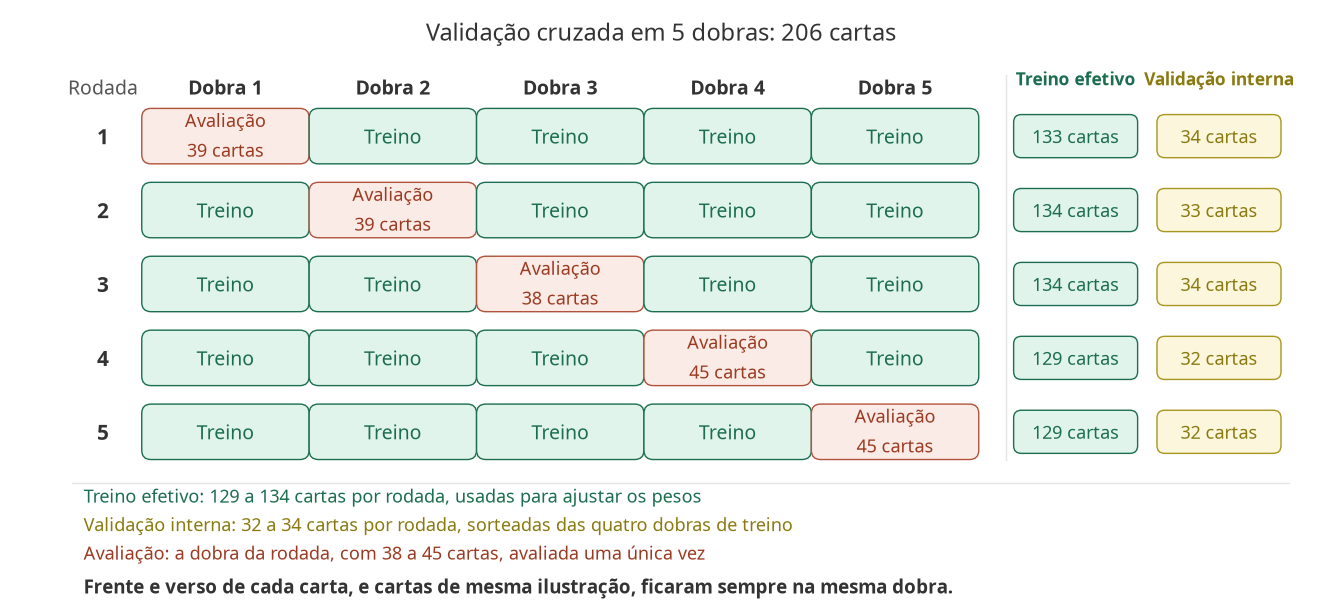
\includegraphics[width=1.00\textwidth]{assets/kfold.png}

    
    \legend{Fonte: Elaborado pelo autor (2026).}
\end{figure}

\subsection{Critérios de validação}
\label{subsec:validacao}

O desempenho de cada rodada foi medido na sua dobra de avaliação. A
métrica usada para testar as hipóteses H1 a H3 foi o F1 por carta
(Seção~\ref{subsec:metricas}), porque a comparação entre as
configurações foi feita carta a carta
(Seção~\ref{subsec:comparacao_estatistica}) e exige uma nota para cada
carta. No seu cálculo, foram consideradas apenas as predições com
confiança igual ou superior ao limiar fixado na validação interna da
rodada (Seção~\ref{subsec:validacao_cruzada}), aplicado sem alteração
à dobra de avaliação. Esse limiar foi o valor de confiança, entre 1.000
valores igualmente espaçados de 0 a 1, que maximizou o F1 agregado da validação interna, calculado pela própria biblioteca, depois de suavizada a curva do F1 em função do
limiar, o mesmo critério que a biblioteca aplica ao conjunto que avalia
\cite{Jocher2023}. Em cada imagem, as predições foram percorridas da
maior para a menor confiança, e cada uma foi associada à anotação ainda
não associada com a qual tinha a maior IoU, desde que essa IoU fosse de
pelo menos 0,5, o mesmo limiar do mAP@0,5; cada associação contou como
verdadeiro positivo, cada predição sem associação como falso positivo e
cada anotação sem predição associada como falso negativo. Os
verdadeiros positivos, os falsos positivos e os falsos negativos da
frente e do verso foram somados, e o F1 da carta foi calculado sobre
essas somas. Assim, as predições feitas em uma face sem anotação contam
como falsos positivos da carta, e uma carta com anotações e sem nenhum
acerto recebe F1 igual a zero. Uma carta sem nenhuma anotação na
referência usada não tem F1 definido e ficou fora das comparações, o
que só ocorreu na anotação sem as caixas sugeridas
(Seção~\ref{subsec:dados}). A revocação por carta foi calculada da
mesma forma.

Além do F1 por carta, foram reportados, para descrever cada
configuração, o mAP@0,5 de cada dobra e a média das cinco dobras, e a
precisão, a revocação e o F1 agregados, obtidos com o mesmo limiar e a
mesma associação, somando os verdadeiros positivos, os falsos positivos
e os falsos negativos de todas as cartas das cinco dobras. As predições
de cada imagem da dobra de avaliação foram salvas com os valores padrão
de avaliação da biblioteca: confiança mínima de 0,001, até 300
predições por imagem e supressão de não máximos, que elimina cada
predição cuja IoU com outra de maior confiança supera 0,7. O mAP@0,5
foi recalculado a partir dessas predições, da mesma forma nas duas
referências de anotação, com a precisão interpolada em 101 valores de
revocação igualmente espaçados, como na biblioteca. Ele não foi usado
para testar hipóteses, porque não fornece uma nota por carta. A precisão e a revocação informadas
pela biblioteca de treinamento não foram usadas, porque correspondem ao
limiar que maximiza o F1 na própria dobra de avaliação. A média e o
desvio padrão entre as cinco dobras não foram usados nos testes das
hipóteses (Seção~\ref{subsec:comparacao_estatistica}).

Cada comparação usou o teste de Wilcoxon pareado bilateral
(Seção~\ref{subsec:comparacao_estatistica}) sobre o F1 por carta, com
as dobras fixas entre as configurações. As comparações que testam H1 a
H3 são as quatro definidas na Seção~\ref{subsec:hipotese}: a
Configuração 2 contra a 1 e a Configuração 4 contra a 3, para H1, e a
Configuração 3 contra a 1 e a Configuração 4 contra a 2, para H2; as
duas que envolvem a Configuração 4 decidem também H3. A elas somou-se
uma quinta, entre a configuração de melhor desempenho, definida
adiante nesta seção, com e sem a cabeça P2. Ela verifica se o acréscimo
da cabeça alterou o desempenho geral do detector, além da revocação
dos defeitos pequenos examinada em H4.

A correção de Holm foi aplicada a essas cinco comparações, isto é,
com $m = 5$, e uma diferença foi considerada significativa quando o
valor-p ajustado ficou abaixo de $\alpha = 0{,}05$. As cinco
comparações foram feitas com as duas referências de anotação, com 206
pares na anotação completa e 201 na anotação sem as caixas sugeridas, e
a correção foi aplicada separadamente em cada referência. Os pares com
diferença nula foram excluídos do cálculo do teste, e seu número é
informado com cada resultado. A revocação por carta foi comparada nas mesmas cinco comparações, com a correção aplicada à parte, para indicar a
origem das diferenças no F1. Cada configuração foi
treinada uma única vez em cada rodada; por isso, o teste trata os
modelos como fixos, como discutido na
Seção~\ref{subsec:comparacao_estatistica}.

A decisão sobre H1, H2 e H3 seguiu uma regra fixa, aplicada em cada referência de anotação. Como o teste é bilateral, uma diferença significativa pode ocorrer nos dois sentidos, e só uma diferença no sentido previsto pela hipótese contou a seu favor. H1 foi considerada confirmada quando as duas comparações correspondentes, a Configuração 2 contra a 1 e a Configuração 4 contra a 3, foram significativas após a correção de Holm, no sentido previsto, e refutada quando alguma delas foi significativa no sentido contrário. Nos demais casos, o resultado foi lido separadamente para cada representação de entrada, como confirmação parcial quando uma das duas comparações foi significativa no sentido previsto e a outra não foi significativa, e como não confirmação quando nenhuma das duas foi significativa. A mesma regra valeu para H2, com as comparações da Configuração 3 contra a 1 e da Configuração 4 contra a 2, lidas separadamente para cada condição de aumento de dados. H3 foi considerada confirmada apenas quando a Configuração 4 superou significativamente as Configurações 2 e 3, refutada quando alguma delas superou significativamente a Configuração 4, e não confirmada nos demais casos.

Como análise adicional, sem hipótese formulada, verificou-se a
interação entre os dois fatores do estudo fatorial
(Seção~\ref{subsec:ablacao_conceito}). Para cada carta, calculou-se o
efeito do aumento de dados com imagens RGB, isto é, o F1 por carta da
Configuração 2 menos o da Configuração 1, e o efeito do aumento de
dados com imagens de realce, o da Configuração 4 menos o da
Configuração 3. Como as variações no espaço HSV só fizeram parte do
aumento de dados das imagens RGB (Seção~\ref{subsec:estrategias}), a
diferença entre esses efeitos inclui também a diferença entre os dois
aumentos de dados. Os dois efeitos foram comparados carta a carta pelo
teste de Wilcoxon pareado bilateral, com a anotação completa: se o
efeito do aumento de dados não depende da representação de entrada, as
diferenças entre eles se distribuem em torno de zero. Essa análise
ficou fora da correção de Holm, por não testar nenhuma das hipóteses.

A ablação e as análises complementares foram feitas sobre a
configuração de melhor desempenho no estudo fatorial. Essa
configuração foi escolhida ao fim do estudo fatorial, como a de maior
mAP@0,5 médio nas cinco dobras de avaliação, com a anotação completa;
ela também obteve o maior F1 agregado. O mAP@0,5 médio foi usado nessa
escolha por ser a métrica de referência dos detectores
(Seção~\ref{subsec:metricas}) e por estar disponível ao fim de cada rodada, sem depender do limiar de confiança.
Essa escolha usou as próprias dobras de avaliação, e não a
validação interna. Como a configuração escolhida serve de referência
nas comparações seguintes, a escolha pode favorecê-la ligeiramente
nelas; as comparações do estudo fatorial não são afetadas, porque seus
pares foram definidos antes, nas hipóteses.

Para H4, cada defeito foi atribuído a uma das três faixas de tamanho da
Seção~\ref{subsec:dados}, pelo menor lado da sua caixa na resolução de
1280 pixels. A associação entre predições e anotações foi a mesma do F1
por carta, feita com todas as anotações da imagem. A revocação de cada
faixa foi o número de defeitos da faixa associados a uma predição,
somado nas cinco dobras de avaliação, dividido pelo total de defeitos
da faixa. A revocação das três faixas foi calculada também para as
quatro configurações do estudo fatorial, como descrição.

O critério de H4, definido na Seção~\ref{subsec:hipotese}, foi a
revocação da faixa abaixo de 8 pixels, com 517 defeitos, comparada
entre a configuração de melhor desempenho com e sem a cabeça P2. Esse
critério não fixou margem mínima de diferença nem teste estatístico.
Como a associação usa o limiar de confiança fixado na validação interna
de cada rodada, os modelos com e sem a cabeça P2 tiveram a revocação
medida em limiares que podem diferir, e um modelo com limiar mais baixo
mantém mais predições e ganha revocação à custa de precisão. Por isso,
o resultado de H4 é lido junto com a comparação do F1 por carta entre
os dois modelos, uma das cinco comparações com correção de Holm, que
leva em conta também a precisão.

Como análise adicional, feita depois dos resultados, a revocação da
faixa abaixo de 8 pixels foi calculada carta a carta nas 127 cartas que
têm ao menos um defeito nela, e os dois modelos foram comparados pelo
teste de Wilcoxon pareado bilateral. Essa análise foi usada apenas para
indicar se a diferença na revocação somada se distingue de uma variação
casual, sem substituir o critério da Seção~\ref{subsec:hipotese}. Todas
essas medidas, inclusive a descrição das quatro configurações, foram
calculadas com as duas referências de anotação; na anotação sem as
caixas sugeridas, a faixa abaixo de 8 pixels tem 513 defeitos, e a
análise por carta reuniu 126 cartas.

A ablação da resolução de entrada e as análises complementares, isto
é, o teste de capacidade e a curva de aprendizado, foram feitas sem
hipótese formulada. Elas usaram a configuração de melhor desempenho, a
anotação completa e dobras isoladas, identificadas de 1 a 5 na ordem
em que foram apresentadas na Seção~\ref{subsec:dados}.

A resolução de entrada de 640 pixels e o YOLOv8m foram avaliados na
Dobra 5, de 45 cartas. Cada um foi comparado com a rodada da
configuração de melhor desempenho nessa dobra, treinada com o YOLOv8s a
1280 pixels, pelo F1 por carta e pelo teste de Wilcoxon pareado
bilateral, com 45 pares e sem correção de Holm.

A curva de aprendizado foi avaliada nas Dobras 3 e 5. Em cada dobra, os
modelos treinados com 25\%, 50\% e 75\% das cartas do treino efetivo e
a rodada com todas elas foram avaliados nas mesmas cartas da dobra de
avaliação, pelo mAP@0,5. A curva usou o mAP@0,5, e não o F1 por carta,
porque o mAP@0,5 não depende do limiar de confiança. Com o F1, cada
ponto da curva teria um limiar próprio, escolhido na validação interna
por um modelo treinado com menos cartas, e a variação dessa escolha
entre os pontos se somaria à variação causada pelo número de cartas de
treino, que é o que a curva mede. A incerteza das diferenças entre os
pontos da curva foi estimada pelo intervalo de confiança por
\textit{bootstrap} descrito na
Seção~\ref{subsec:comparacao_estatistica}, com a carta como unidade
sorteada. Em cada repetição, a mesma amostra de cartas foi usada para
recalcular o mAP@0,5 de todos os pontos. O intervalo foi obtido para a
diferença entre pontos consecutivos e entre 50\% e 100\% das cartas do
treino efetivo.

A Tabela~\ref{tab:plano_experimentacao} resume os experimentos, com o
que variou e o que ficou fixo em cada um, as dobras usadas e a métrica
e o teste de cada comparação.

\begin{table}[htb]
\centering
\caption{Plano de experimentação}
\label{tab:plano_experimentacao}
\scriptsize
\setlength{\tabcolsep}{4pt}
\begin{tabular}{>{\raggedright\arraybackslash}p{2.0cm}>{\raggedright\arraybackslash}p{2.0cm}>{\raggedright\arraybackslash}p{2.3cm}>{\raggedright\arraybackslash}p{2.7cm}>{\raggedright\arraybackslash}p{1.3cm}>{\raggedright\arraybackslash}p{3.6cm}}
\toprule
\textbf{Experimento} & \textbf{Objetivo} & \textbf{O que varia} & \textbf{O que fica fixo} & \textbf{Dobras} & \textbf{Métrica e teste} \\
\midrule
Escolha da variante de realce & Escolher a variante das Configurações 3 e 4; sem hipótese & Variante de realce de micro-relevo (quatro) & Configuração 3, YOLOv8s, 1280 pixels & Dobra 1 & F1 agregado na validação interna, calculado pela biblioteca; escolhida a variante de maior valor, sem teste \\
\midrule
Estudo fatorial $2 \times 2$ & H1, H2 e H3 & Aumento de dados (sem ou com) e representação de entrada (RGB ou realce) & YOLOv8s com pesos pré-treinados, 1280 pixels, demais hiperparâmetros e dobras & 1 a 5 & F1 por carta; Wilcoxon pareado bilateral (206 e 201 pares), com correção de Holm; interação como análise adicional \\
\midrule
Ablação da cabeça P2 & H4 & Cabeça P2 (sem ou com) & Configuração de melhor desempenho e demais condições do estudo fatorial & 1 a 5 & H4: revocação somada dos defeitos menores que 8 pixels, sem teste; F1 por carta com Wilcoxon e Holm; revocação por carta nessa faixa com Wilcoxon, como análise adicional \\
\midrule
Ablação da resolução de entrada & Sem hipótese & 640 ou 1280 pixels & Configuração de melhor desempenho, YOLOv8s & Dobra 5 & F1 por carta; Wilcoxon pareado bilateral (45 pares), sem Holm \\
\midrule
Curva de aprendizado & Análise complementar, sem hipótese & Fração das cartas do treino efetivo (25\%, 50\%, 75\% e 100\%) & Configuração de melhor desempenho, YOLOv8s, 1280 pixels & Dobras 3 e 5 & mAP@0,5, que não depende do limiar de confiança; intervalo de confiança de 95\% por \textit{bootstrap} percentil, com a carta como unidade \\
\midrule
Teste de capacidade & Análise complementar, sem hipótese & YOLOv8s ou YOLOv8m & Configuração de melhor desempenho, 1280 pixels & Dobra 5 & F1 por carta; Wilcoxon pareado bilateral (45 pares), sem Holm \\
\bottomrule
\end{tabular}
\legend{Dobras numeradas de 1 a 5 na ordem da Seção~\ref{subsec:dados}. Em todos os experimentos, o limiar de confiança foi fixado na validação interna de cada rodada, a associação entre predição e anotação exigiu IoU de pelo menos 0,5, e o mAP@0,5, a precisão, a revocação e o F1 agregados foram reportados como descrição.
Fonte: Elaborado pelo autor (2026).}
\end{table}

% ---------------------------------------------------------------
\section{Detalhes da implementação}
\label{sec:implementacao}

Esta seção descreve o modelo usado nos experimentos
(Seção~\ref{subsec:modelo_base}), os hiperparâmetros de treinamento,
inclusive os de aumento de dados de cada configuração
(Seção~\ref{subsec:hiperparametros}), e o ambiente computacional em que
os treinamentos foram executados (Seção~\ref{subsec:ferramentas}).

\subsection{Modelo base}
\label{subsec:modelo_base}

As rodadas usaram o YOLOv8s, a variante \textit{small} do YOLOv8,
inicializado com os pesos pré-treinados no COCO disponibilizados pela
biblioteca Ultralytics (Seção~\ref{subsec:yolo}) e submetido a ajuste
fino sobre as imagens das cartas, com a classe única \textit{defeito}.
Nenhuma camada foi congelada: todos os pesos foram ajustados durante o
treinamento. Houve duas exceções ao uso do YOLOv8s com todos os pesos
pré-treinados, descritas adiante nesta seção: o teste de capacidade
usou o YOLOv8m, e a ablação da cabeça P2 usou uma versão do YOLOv8s
que recebeu os pesos pré-treinados em
apenas parte das camadas. Os pesos iniciais foram os mesmos em todas
as configurações: o \textit{transfer learning} não foi um fator do
estudo, mas a base comum sobre a qual o aumento de dados e o realce de
micro-relevo foram comparados.

O YOLOv8 foi mantido como detector, em vez de versões mais recentes da
família YOLO, por três motivos. Primeiro, foi a arquitetura definida
antes dos experimentos e usada nos testes preliminares, que verificaram
a viabilidade do protocolo no equipamento disponível
(Seção~\ref{subsec:visao_geral}). Segundo, é a versão usada pelos dois
trabalhos correlatos que tratam de detecção de objetos
(Seção~\ref{sec:trabalhos_correlatos}), o que aproxima as condições
deste trabalho das deles. Terceiro, a biblioteca utilizada oferece para
o YOLOv8 uma variante oficial com a cabeça de detecção P2, necessária à
ablação, o que permitiu fazê-la sem modificar a arquitetura por conta
própria \cite{Jocher2023}.

Entre os tamanhos do YOLOv8, adotou-se o \textit{small}, com cerca de
11 milhões de parâmetros, pelo custo de memória e de tempo. Com a
configuração de treinamento descrita na
Seção~\ref{subsec:hiperparametros}, o YOLOv8s ocupou cerca de 7,1 GB
dos 16 GB de memória da placa de vídeo e levou cerca de 28 segundos por
época. O tamanho seguinte, o YOLOv8m, com cerca de 26 milhões de
parâmetros \cite{Jocher2023}, ocupou 11,6 GB e levou 58 segundos por
época na rodada em que foi treinado. O acréscimo da cabeça P2 elevou
a memória ocupada pelo YOLOv8s em cerca de 4 a 6 GB, conforme a dobra;
somado aos 11,6 GB do YOLOv8m, um acréscimo dessa ordem deixaria a
ocupação no limite dos 16 GB da placa ou acima deles, e a combinação do
YOLOv8m com a cabeça P2 não foi treinada. A possibilidade de que a capacidade
do YOLOv8s limitasse o desempenho foi examinada pelo teste de
capacidade (Tabela~\ref{tab:plano_experimentacao}), cujo resultado é
apresentado na Seção~\ref{sec:resultados}.

Na ablação da cabeça P2, usou-se a variante P2 do YOLOv8s oferecida
pela biblioteca (Seção~\ref{subsec:objetos_pequenos}), com os mesmos
pesos pré-treinados, dobras e hiperparâmetros da configuração sem a
cabeça P2. A biblioteca só transfere os pesos de uma camada quando o
nome, que inclui a posição da camada na rede, e o formato coincidem nos
dois modelos. O \textit{backbone} e o caminho de cima para baixo do
\textit{neck} até o nível P3 são iguais nas duas arquiteturas e
receberam os pesos pré-treinados. As camadas acrescentadas para levar
as características até o nível P2 deslocaram a posição das seguintes;
por isso, o caminho de baixo para cima do \textit{neck}, exceto poucos
conjuntos de pesos que coincidiram por acaso, e toda a cabeça de detecção,
inclusive nos níveis P3 a P5, começaram com valores aleatórios. Ao
todo, foram transferidos 219 dos 437 tensores de pesos do modelo, isto
é, dos conjuntos de valores aprendidos de suas camadas. Essa perda de
pré-treino, prevista na Seção~\ref{subsec:transfer_learning},
acompanhou todas as rodadas com a cabeça P2 e é considerada na análise
dos resultados. Com essa cabeça, a memória ocupada ficou entre 11,2 e
13,1 GB, e o tempo por época, entre 41 e 43 segundos.

\subsection{Hiperparâmetros de treinamento}
\label{subsec:hiperparametros}

Os hiperparâmetros de treinamento foram os mesmos em todas as rodadas,
exceto o elemento que cada experimento variou
(Tabela~\ref{tab:plano_experimentacao}); os parâmetros de aumento de
dados, que definem um dos fatores do estudo fatorial, são apresentados
adiante. A resolução
de entrada foi de 1280 pixels, a mesma dos testes preliminares, e a
distribuição do tamanho dos defeitos na anotação final
(Tabela~\ref{tab:tamanho_defeitos}) sustentou a escolha: nela, a fração das
anotações com menor lado abaixo do passo do nível P3 cai de 57,6\%, a
640 pixels, para 10,8\%. Como o lado maior da maior parte das
imagens recortadas supera 1280 pixels (Seção~\ref{subsec:dados}), o
aumento de tamanho corresponde a detalhe presente na fotografia. O
custo também aumenta: na Dobra 5, a rodada da configuração de melhor
desempenho a 640 pixels ocupou 2,1 GB da memória da placa de vídeo e
levou 7,7 segundos por época, contra 7,1 GB e 27,7 segundos a 1280
pixels.

As imagens foram processadas em lotes de 4. A biblioteca
acumula o resultado de 16 lotes antes de cada atualização dos pesos,
de modo que cada atualização considerou 64 imagens. Lotes de 8 imagens
foram experimentados nos testes preliminares e travaram a placa de
vídeo nas duas tentativas, por falha da biblioteca da AMD que executa as
convoluções, e não por falta de memória, já que a ocupação estimada, de
cerca de 12,5 GB, caberia nos 16 GB da placa.

O otimizador, algoritmo que calcula o ajuste dos pesos a cada
atualização, foi escolhido pela própria biblioteca, na opção
automática: para treinamentos com até 10 mil atualizações, como os
deste trabalho, ela adota o AdamW, com taxa de aprendizado inicial, que
regula o tamanho de cada ajuste, de 0,002 quando há uma única classe
\cite{Jocher2023}. Os demais hiperparâmetros de otimização mantiveram o
valor padrão da biblioteca. O treinamento usou semente aleatória fixa e
o modo determinístico da biblioteca, e cada configuração foi treinada
uma única vez em cada rodada. Duas rodadas interrompidas foram
retomadas a partir do estado salvo ao fim da última época concluída,
com os mesmos parâmetros.

Cada rodada teve teto de 300 épocas e parada antecipada com paciência
de 100 épocas: o treino foi interrompido quando a validação interna
passou 100 épocas sem melhora, e foram mantidos os pesos da melhor
época (Seção~\ref{subsec:validacao_cruzada}). A melhora foi medida pelo
critério da biblioteca, que, na versão usada, é o mAP@0,5:0,95 na
validação interna \cite{Jocher2023}, e não o mAP@0,5. Nenhuma rodada
atingiu o teto de 300 épocas: todas foram encerradas pela paciência.

A paciência de 100 épocas, que coincide com o valor padrão da
biblioteca, foi usada também nos testes preliminares. \citeonline{Prechelt1998} observa que critérios
de parada mais lentos trazem pequena melhora na generalização ao custo
de cerca de quatro vezes mais tempo de treinamento; neste trabalho,
esse custo coube no cronograma, e uma escolha ruim do ponto de parada
acrescentaria variação às comparações entre as configurações.

Os hiperparâmetros de aumento de dados foram definidos por
configuração, conforme a Tabela~\ref{tab:augmentation}. A biblioteca
aplica, por padrão, sete transformações de aumento de dados no
treinamento de detectores: o mosaico (\texttt{mosaic}), a variação de
escala (\texttt{scale}), a translação (\texttt{translate}), o
espelhamento horizontal (\texttt{fliplr}) e as três variações no espaço
HSV (\texttt{hsv\_h}, \texttt{hsv\_s} e \texttt{hsv\_v})
\cite{Jocher2023}. Por isso, a ausência de aumento de dados nas
Configurações 1 e 3 exigiu o desligamento explícito desses parâmetros:
com os valores padrão, essas configurações receberiam mais
transformações do que as Configurações 2 e 4, o que inverteria o
sentido do fator investigado no estudo fatorial. Nas Configurações 2 e
4, as transformações mantidas conservaram o valor padrão da biblioteca,
e acrescentou-se a rotação de até 10 graus, uma das transformações geométricas de aumento de dados apresentadas na Seção~\ref{subsec:data_augmentation}, em valor que não foi ajustado por teste. Ao girar a imagem, a biblioteca
substitui cada caixa pela menor caixa alinhada aos eixos que contém os
seus quatro cantos girados, o que a alarga; o efeito é maior nas 367
caixas em forma de faixa (Seção~\ref{subsec:dados}): no ângulo máximo,
uma faixa de 100 por 5 pixels passa a ser representada por uma caixa de
cerca de 99 por 22 pixels. Na Configuração 4, as
variações no espaço HSV foram desligadas, porque o realce de
micro-relevo já ajusta o contraste local pelo CLAHE e seus três canais
não representam cores (Seção~\ref{subsec:fotometria}); variações
artificiais de cor e de brilho perturbariam o sinal que ele constrói.

Dois parâmetros foram desligados em todas as configurações, inclusive
nas com aumento de dados. O primeiro é a variação de escala. No valor
padrão de 0,5, ela multiplica o tamanho da imagem por um fator sorteado
entre 0,5 e 1,5, isto é, pode reduzi-la até a metade ou ampliá-la em
até 50\%. Reduzir à metade uma imagem de 1280 pixels deixa os defeitos com o tamanho que
teriam na resolução de 640 pixels, na qual 57,6\% das anotações ficam
abaixo do passo do nível P3 (Tabela~\ref{tab:tamanho_defeitos}); a
transformação desfaria, em parte das imagens de treino, o ganho da
resolução de entrada adotada. A biblioteca permite restringir o sorteio
a fatores de ampliação, mas essa opção, que também levaria parte da
carta para fora da imagem, não foi avaliada.

O segundo é o mosaico, que combina quatro imagens e recorta delas uma
janela do tamanho da entrada (Seção~\ref{subsec:data_augmentation}).
Com a variação de escala desligada, ele não reduz os objetos. O
recorte, porém, pode cortar defeitos nas bordas de cada imagem, e a imagem resultante reúne partes de
quatro cartas, situação que não ocorre na avaliação, feita sobre a
carta inteira. A translação, mantida nas Configurações 2 e 4, também
pode levar para fora da imagem uma faixa da carta de até 10\% da
altura, e com ela parte do desgaste da borda superior ou inferior; a biblioteca corta as
caixas no limite da imagem e descarta as que perdem mais de 90\% da
área. A perda é menor que no mosaico, do qual cada imagem participa
apenas com a parte que cai na janela recortada. Os demais parâmetros de aumento de dados que a
biblioteca aplica ao treinamento de detectores já valem zero por padrão e foram mantidos assim em todas as
configurações.

Os valores da Tabela~\ref{tab:augmentation} ficaram fixos nas cinco
dobras de cada configuração. As transformações foram aplicadas apenas
às imagens de treino de cada rodada, no momento em que cada imagem era
carregada, e nunca gravadas em disco antes da divisão em dobras; assim,
versões transformadas de uma carta não puderam aparecer no treino e na
avaliação ao mesmo tempo. O pacote opcional Albumentations não foi
instalado, porque, quando ele está presente, a biblioteca o usa para
aplicar desfoque, conversão para tons de cinza e equalização de
contraste a uma pequena parte das imagens de todas as configurações,
inclusive das que não têm aumento de dados.

\begin{table}[htb]
\centering
\caption{Parâmetros de aumento de dados por configuração}
\label{tab:augmentation}
\footnotesize
\begin{tabular}{lcccc p{4.2cm}}
\toprule
 & & \multicolumn{3}{c}{\textbf{Configuração}} & \\
\cmidrule(lr){3-5}
\textbf{Parâmetro} & \textbf{Padrão} & \textbf{1 e 3} & \textbf{2} & \textbf{4} & \textbf{Motivo do valor adotado} \\
\midrule
\texttt{hsv\_h}    & 0,015 & 0,0 & 0,015 & 0,0  & Configuração 4: realce com contraste ajustado pelo CLAHE e canais que não são cores \\
\texttt{hsv\_s}    & 0,7   & 0,0 & 0,7   & 0,0  & idem \\
\texttt{hsv\_v}    & 0,4   & 0,0 & 0,4   & 0,0  & idem \\
\texttt{degrees}   & 0,0   & 0,0 & 10,0  & 10,0 & transformação geométrica usual, valor não ajustado; alarga as caixas em faixa \\
\texttt{translate} & 0,1   & 0,0 & 0,1   & 0,1  & padrão mantido \\
\texttt{fliplr}    & 0,5   & 0,0 & 0,5   & 0,5  & padrão mantido \\
\texttt{mosaic}    & 1,0   & 0,0 & 0,0   & 0,0  & corta defeitos nas bordas e reúne partes de quatro cartas \\
\texttt{scale}     & 0,5   & 0,0 & 0,0   & 0,0  & a redução leva defeitos para baixo do passo do nível P3 \\
\midrule
\multicolumn{6}{p{13.5cm}}{\footnotesize \texttt{shear}, \texttt{perspective}, \texttt{flipud}, \texttt{bgr}, \texttt{mixup}, \texttt{cutmix} e \texttt{copy\_paste} ficaram em 0,0 em todas as configurações, valor que já é o padrão da biblioteca.} \\
\bottomrule
\end{tabular}
\legend{Padrão: valor padrão da biblioteca Ultralytics 8.4.138. Nas Configurações 1 e 3, sem aumento de dados, todos os parâmetros foram zerados; nas Configurações 2 e 4, os valores diferentes do padrão estão justificados na última coluna.
Fonte: Elaborado pelo autor (2026).}
\end{table}

\subsection{Tecnologias e ferramentas}
\label{subsec:ferramentas}

A implementação foi feita em Python, versão 3.12. O treinamento e a
avaliação dos modelos usaram a biblioteca Ultralytics, versão 8.4.138,
que mantém a implementação de referência do YOLOv8 e oferece a variante
com a cabeça P2 \cite{Jocher2023}, sobre o PyTorch 2.14.0 com a
plataforma ROCm 7.2, que permite executar o PyTorch em placas de vídeo
AMD, como a do equipamento disponível; a versão anterior testada, o PyTorch
2.10.0 com a plataforma ROCm 7.0, falhou durante o treinamento nessa
placa. O recorte automático da
carta e a geração das imagens de realce de micro-relevo usaram a
biblioteca OpenCV, versão 5.0, que oferece a conversão entre espaços de
cor, os filtros e o CLAHE empregados, e a biblioteca NumPy, versão 2.5,
nas operações sobre matrizes, como o cálculo da medida de Frangi; os
testes estatísticos usaram a biblioteca SciPy, versão 1.18, que
implementa o teste de Wilcoxon pareado. Os experimentos foram executados em um computador
com o sistema operacional Ubuntu 24.04 e placa de vídeo AMD Radeon RX
9060 XT, com 16 GB de memória. A lista completa de pacotes e versões
acompanha o código do trabalho, disponível em repositório
público\footnote{\url{https://github.com/Marynxs/tcc-deteccao-defeitos-pokemon-tcg-yolov8}}.

% ---------------------------------------------------------------
\section{Experimentos e cenário de testes}
\label{sec:experimentos}

Esta seção define as quatro configurações comparadas no estudo
fatorial e descreve como as imagens de realce de micro-relevo foram
geradas e como a variante adotada foi escolhida
(Seção~\ref{subsec:estrategias}); em seguida, descreve as rodadas de
treinamento do estudo fatorial, da ablação e das análises
complementares (Seção~\ref{subsec:ablacao}).

\subsection{Estratégias de treinamento avaliadas}
\label{subsec:estrategias}

O estudo fatorial (Seção~\ref{subsec:ablacao_conceito}) cruzou dois
fatores: o aumento de dados, sem ou com, e a representação de entrada,
imagens RGB ou imagens de realce de micro-relevo. As quatro
combinações formaram as configurações comparadas:

\begin{description}
    \item[Configuração 1] imagens RGB, sem aumento de dados;
    \item[Configuração 2] imagens RGB, com aumento de dados;
    \item[Configuração 3] imagens de realce de micro-relevo, sem aumento
    de dados;
    \item[Configuração 4] imagens de realce de micro-relevo, com aumento
    de dados.
\end{description}

As quatro configurações usaram o mesmo modelo, os mesmos pesos
pré-treinados e os mesmos hiperparâmetros de treinamento, exceto os de
aumento de dados (Seção~\ref{sec:implementacao}); a Configuração 1
corresponde, assim, ao ajuste fino sem nenhuma das duas estratégias. As
hipóteses H1 e H2 (Seção~\ref{subsec:hipotese}) tratam do efeito de
cada fator, e H3, da combinação dos dois na Configuração 4; as
comparações que testaram cada uma estão na
Seção~\ref{subsec:validacao}.

Nas Configurações 2 e 4, o aumento de dados aplicou às imagens de
treino a translação, o espelhamento horizontal e a rotação; na
Configuração 2, aplicou também as variações de matiz, saturação e valor
no espaço HSV, que ficaram desligadas na Configuração 4 pelo motivo
exposto na Seção~\ref{subsec:hiperparametros}. Os valores de cada
parâmetro estão na Tabela~\ref{tab:augmentation}, e a consequência
dessa diferença para a comparação entre as representações de entrada
é discutida adiante, nesta seção.

As imagens de realce de micro-relevo das Configurações 3 e 4 foram
geradas a partir das imagens recortadas (Seção~\ref{subsec:dados}),
sempre a partir do canal de luminosidade (L$^*$) do espaço CIELAB, com
os operadores apresentados na Seção~\ref{subsec:fotometria}, aplicados
na resolução da imagem recortada, antes da redução à resolução de
entrada. Quatro variantes foram comparadas:

\begin{description}
    \item[\textit{Emboss} e CLAHE] o filtro \textit{emboss}, com núcleo
    de $3 \times 3$ pixels cujas linhas são $(-2, -1, 0)$, $(-1, 0, 1)$
    e $(0, 1, 2)$, que responde à variação de luminosidade na direção
    diagonal; a resposta, somada a 128 e limitada à faixa de 0 a 255,
    foi seguida do CLAHE;
    \item[CLAHE e \textit{emboss} em oito direções] o CLAHE seguido do
    filtro \textit{emboss} aplicado em oito direções, como no trabalho
    sobre superfícies pintadas discutido na
    Seção~\ref{subsec:fotometria}, mantendo-se em cada pixel a maior
    resposta em valor absoluto; as oito direções foram obtidas girando
    os coeficientes da borda do mesmo núcleo uma posição por vez, em
    passos de 45 graus, e, como direções opostas dão o mesmo valor
    absoluto, correspondem a quatro eixos distintos;
    \item[Frangi] o CLAHE seguido da medida de Frangi, calculada com
    núcleos gaussianos de desvio padrão de 1,5, 3 e 5 pixels,
    mantendo-se em cada pixel a maior resposta entre essas escalas;
    \item[Composição de três canais] a variante descrita na
    Seção~\ref{subsec:fotometria}, em que os três canais de entrada
    recebem a luminosidade original, a luminosidade com CLAHE e a medida
    de Frangi da variante anterior.
\end{description}

Nas três primeiras variantes, a imagem resultante, de um único canal,
foi repetida nos três canais de entrada da rede; na última, cada canal
recebeu uma informação diferente. Em todas, o CLAHE usou uma grade de
$8 \times 8$ ladrilhos, valor padrão da biblioteca OpenCV, e limite de
corte de 3,0, mais baixo que o padrão da biblioteca, de 40, o que torna
o realce mais suave. Esses valores não foram ajustados por teste, e a
medida de Frangi usou os parâmetros indicados por seus autores
(Seção~\ref{subsec:fotometria}).

As respostas do \textit{emboss} em oito
direções e da medida de Frangi foram convertidas para a faixa de
intensidades de 0 a 255, por uma escala linear que leva o percentil 1
ao valor 0 e o percentil 99,5 ao valor 255, percentis calculados em
cada imagem; os valores fora desse intervalo foram fixados nesses
limites. A medida de Frangi foi implementada pelo autor. Em cada
escala, a imagem foi suavizada pelo núcleo gaussiano, e as derivadas
de segunda ordem foram aproximadas por diferenças em uma vizinhança de
$3 \times 3$ pixels e multiplicadas pelo quadrado do desvio padrão,
para tornar comparáveis as respostas das escalas. A medida foi
calculada a partir dos autovalores da Hessiana assim obtida, sem
distinguir estruturas mais claras ou mais escuras que a vizinhança, já
que a carta tem defeitos dos dois tipos.

As escalas da medida de Frangi e o núcleo do \textit{emboss} foram
definidos em pixels da imagem recortada, e não em proporção da carta.
Como a resolução das fotografias varia, a mesma escala corresponde a estruturas de tamanhos
diferentes na carta. A variação é limitada, porque 317 das 412 imagens
foram recebidas na mesma resolução, de $1280 \times 1771$ pixels
(Seção~\ref{subsec:dados}).

A variante foi escolhida uma única vez, antes do estudo fatorial, na
rodada da Dobra 1. A Configuração 3 foi treinada com cada uma das
quatro variantes, com os demais hiperparâmetros iguais aos das outras
rodadas. Foi adotada nas Configurações 3 e 4 a variante de maior F1
agregado na validação interna dessa rodada, calculado com a anotação
completa pela própria biblioteca de treinamento. A biblioteca escolhe o limiar no próprio conjunto em que mede o F1, aqui a validação interna, e associa predições e anotações percorrendo os pares em ordem decrescente de IoU, e não as predições em ordem decrescente de confiança. No procedimento da Seção~\ref{subsec:validacao}, o limiar escolhido na validação interna foi aplicado à dobra de avaliação, com a associação descrita naquela seção.

A composição de três canais obteve F1 de 0,208; o
\textit{emboss} seguido do CLAHE, 0,192; a medida de Frangi, 0,161; e o
CLAHE seguido do \textit{emboss} em oito direções, 0,151. A vantagem da
variante adotada sobre a segunda foi de 8\% do valor desta e, no
mAP@0,5 da mesma validação interna, também calculado pela biblioteca,
de 2\%. Como cada variante foi
treinada uma única vez, em uma única dobra, essa diferença não foi
testada e não permite afirmar que a composição de três canais seja
superior às demais: a escolha foi uma seleção de hiperparâmetro, e não
um resultado do trabalho.

A escolha também não ficou isolada das rodadas seguintes. As 34 cartas
da validação interna da Dobra 1 pertencem às outras quatro dobras e
foram, portanto, avaliadas nas rodadas correspondentes. Como a variante
adotada foi a de maior F1 justamente nessas cartas, a escolha pode
favorecer ligeiramente as Configurações 3 e 4 nas comparações com as
Configurações 1 e 2 (Seção~\ref{subsec:validacao_cruzada}).

A comparação entre as duas representações de entrada não isola apenas
o realce de micro-relevo, por dois motivos. Primeiro, o aumento de
dados não foi idêntico nas duas: as variações no espaço HSV só foram
aplicadas às imagens RGB, de modo que a comparação entre as
Configurações 2 e 4 difere também na presença dessas variações, e o
efeito do aumento de dados medido com imagens RGB inclui
transformações que não foram aplicadas às imagens de realce. Segundo,
as quatro variantes partem apenas da luminosidade (L$^*$) e descartam
os dois canais de cor do espaço CIELAB. Assim, as comparações entre as
Configurações 3 e 1 e entre as Configurações 4 e 2 opõem também
imagens com cor a imagens sem cor. Uma representação de controle, com
a luminosidade sem realce repetida nos três canais, não foi treinada;
por isso, uma diferença entre as imagens RGB e as de realce pode
decorrer tanto do realce quanto da retirada da cor.

A Figura~\ref{fig:rgb_fotometrica} mostra uma carta do conjunto de
dados em RGB e na composição de três canais adotada.

\begin{figure}[H]
    \centering
    \caption{Carta do conjunto de dados em RGB e na variante de realce de micro-relevo adotada nas Configurações 3 e 4}
    \label{fig:rgb_fotometrica}
    \begin{minipage}{0.45\textwidth}
        \centering
        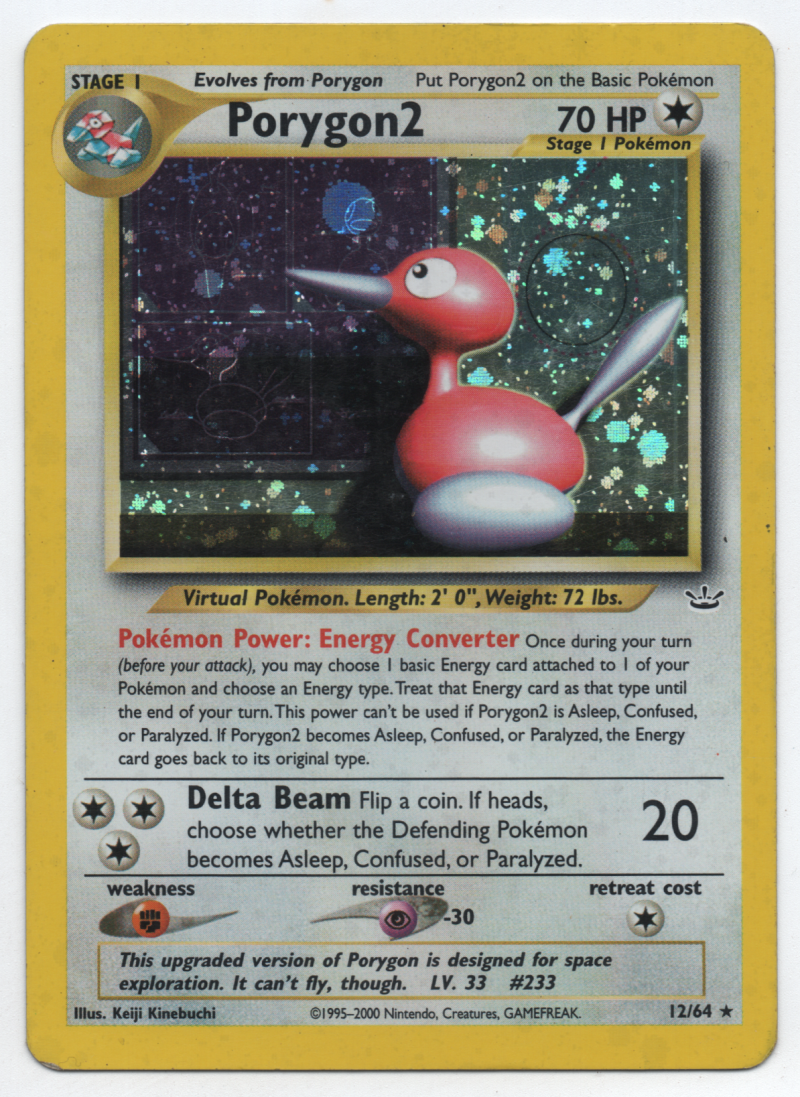
\includegraphics[width=0.90\textwidth]{assets/realce_carta070_rgb.png}

        \vspace{0.2cm}
        {\small (a) Imagem RGB}
    \end{minipage}
    \hfill
    \begin{minipage}{0.45\textwidth}
        \centering
        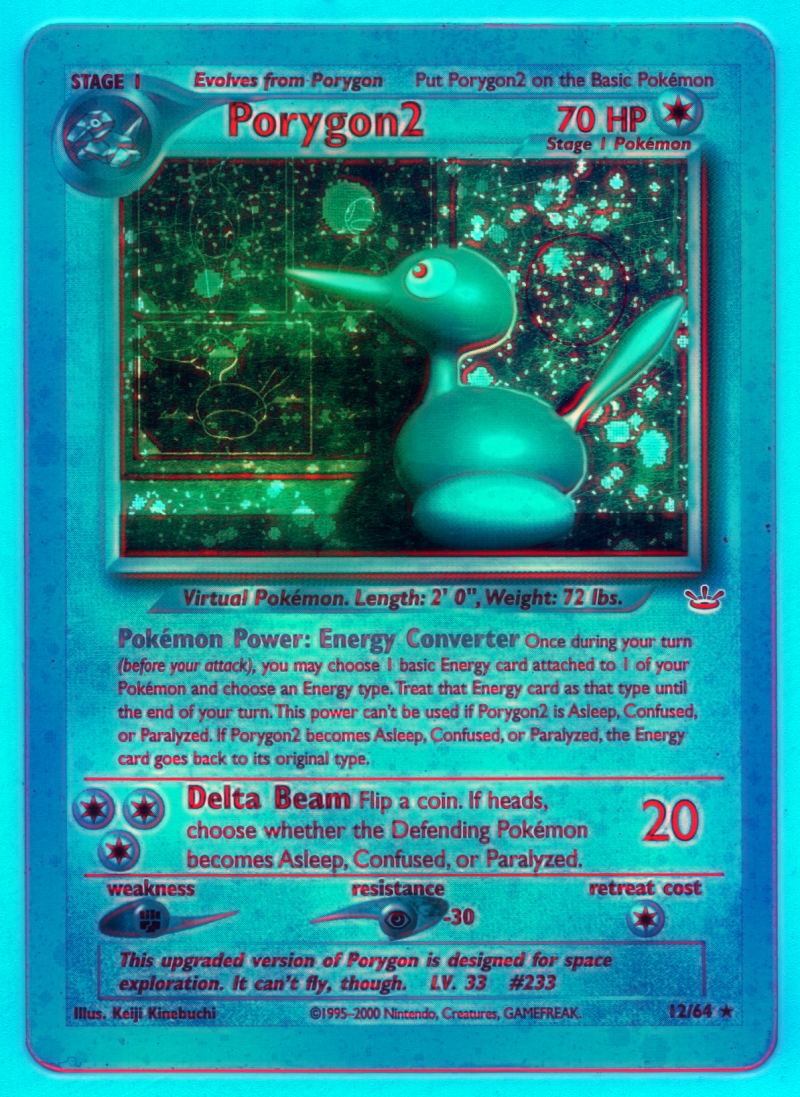
\includegraphics[width=0.90\textwidth]{assets/realce_carta070_composicao.png}

        \vspace{0.2cm}
        {\small (b) Composição de três canais}
    \end{minipage}

    \legend{Na imagem (b), exibida como imagem colorida, os canais azul, verde e vermelho contêm, respectivamente, a luminosidade, a luminosidade com CLAHE e a medida de Frangi; as cores não têm significado para a rede.
Fonte: Imagem RGB fornecida pela empresa de graduação; imagem de realce elaborada pelo autor a partir dela (2026).}
\end{figure}

\subsection{Estudo fatorial, ablação e análises complementares}
\label{subsec:ablacao}

O estudo fatorial, a ablação e as análises complementares seguiram as
etapas da Seção~\ref{subsec:visao_geral} e o plano da
Tabela~\ref{tab:plano_experimentacao}. As 20 rodadas do estudo
fatorial, das quatro configurações nas cinco dobras, usaram o YOLOv8s a
1280 pixels e as mesmas dobras. A ablação e as análises complementares
partiram da configuração de melhor desempenho e alteraram um único
elemento por vez, mantendo os demais iguais aos da rodada do estudo
fatorial na mesma dobra. Os elementos alterados foram a cabeça P2, nas
cinco dobras, que trouxe junto a perda dos pesos pré-treinados em parte
das camadas (Seção~\ref{subsec:modelo_base}); a resolução de entrada de
640 pixels e o YOLOv8m, cada um em uma rodada na Dobra 5; e a fração
das cartas do treino efetivo, na curva de aprendizado. Ao todo,
contadas as quatro rodadas da escolha da variante de realce, foram 37
rodadas de treinamento.

Na curva de aprendizado, a configuração de melhor desempenho foi
treinada com 25\%, 50\% e 75\% das cartas do treino efetivo, nas
Dobras 3 e 5, com a validação interna e a dobra de avaliação
inalteradas; o ponto de 100\% é a rodada do estudo fatorial na mesma
dobra. As cartas foram sorteadas uma única vez, com semente fixa, de
modo que cada fração contivesse a anterior e que as cartas de mesma
ilustração ficassem juntas.

As dobras da ablação da resolução e das análises complementares foram escolhidas depois do estudo fatorial. A
Dobra 5 foi escolhida por ter, na avaliação, o número de anotações mais
próximo do típico entre as cinco dobras (783, a mediana) e por não
conter as cartas de desgaste mais extenso, que ficaram nas Dobras 1 e
4; nela, a configuração de melhor desempenho teve o maior mAP@0,5 entre
as cinco dobras. Se parte desse valor se deve à variação da própria
rodada, e não apenas a uma dobra mais fácil, a rodada de referência
está acima do seu desempenho típico, e as diferenças medidas contra ela
tendem a favorecê-la: a vantagem de 1280 sobre 640 pixels pode estar
exagerada, e a comparação com o YOLOv8m pode estar desfavorável a ele.
A resolução de 640 pixels e o YOLOv8m foram avaliados na mesma dobra, o
que permitiu compará-los com a mesma rodada de referência da curva. A
curva de aprendizado foi repetida na Dobra 3, que, como a 5, não contém
as cartas de desgaste mais extenso, para verificar se sua forma se
mantinha em outra dobra.

% ---------------------------------------------------------------
\section{Resultados e análises}
\label{sec:resultados}

% A ESCREVER: resultados das quatro configuracoes, analise critica e
% discussao. Depende da execucao dos experimentos.

% ===============================================================
% CAPÍTULO 4 - CONCLUSÃO
% ===============================================================
\chapter{Conclusão}
\label{cap:conclusao}

\section{Retomada do problema e dos objetivos}
% A ESCREVER

\section{Contribuições para a Computação}
% A ESCREVER

\section{Limitações e trabalhos futuros}
% A ESCREVER

% ---------------------------------------------------------------
% ELEMENTOS PÓS-TEXTUAIS
% ---------------------------------------------------------------
\postextual

% ===============================================================
% REFERÊNCIAS BIBLIOGRÁFICAS
% ===============================================================
\bibliography{bibliografia_tcc2}

% ---------------------------------------------------------------
% APÊNDICES
% ---------------------------------------------------------------
\begin{apendicesenv}
\partapendices

\chapter{Cronograma previsto no TCC1}
\label{ap:cronograma}

O cronograma de trabalho organiza as principais atividades previstas para o desenvolvimento do TCC2, contemplando desde a preparação final do conjunto de dados até a execução dos experimentos, análise dos resultados e redação da versão final do trabalho. As etapas foram distribuídas de forma sequencial, considerando a dependência entre a organização dos dados, o treinamento dos modelos, a comparação das configurações experimentais e a consolidação dos resultados obtidos.

\begin{figure}[htb]
    \centering
    \caption{Cronograma de atividades do TCC2 para o segundo semestre de 2026 -- Diagrama de Gantt}
    \label{fig:gantt}
    \begin{ganttchart}[
        hgrid,
        vgrid,
        x unit=0.68cm,
        y unit title=0.6cm,
        y unit chart=1cm,
        title height=1,
        bar height=0.45,
        bar label font=\scriptsize,
        group label font=\scriptsize\bfseries,
        title label font=\small,
        milestone label font=\scriptsize\itshape,
        bar/.append style={fill=blue!40},
        group/.append style={draw=black, fill=blue!70},
        milestone/.append style={fill=red!70},
        bar label node/.append style={text width=3.8cm, align=right},
        group label node/.append style={text width=3.8cm, align=right},
        milestone label node/.append style={text width=3.8cm, align=right}
    ]{1}{16}
        \gantttitle{Segundo semestre de 2026}{16} \\
        \gantttitle{Semanas}{16} \\
        \gantttitlelist{1,...,16}{1} \\

        \ganttgroup{Fase 1: Preparação experimental}{1}{4} \\
        \ganttbar{Revisão da literatura e metodologia}{1}{2} \\
        \ganttbar{Revisão das anotações do dataset}{2}{4} \\
        \ganttbar{Particionamento dos dados}{3}{4} \\
        \ganttmilestone{Base preparada}{4} \\

        \ganttgroup{Fase 2: Implementação do pipeline}{5}{7} \\
        \ganttbar{Configuração do ambiente}{5}{5} \\
        \ganttbar{Implementação do YOLOv8 base}{5}{6} \\
        \ganttbar{Ajuste de hiperparâmetros}{6}{7} \\
        \ganttmilestone{Pipeline validado}{7} \\

        \ganttgroup{Fase 3: Execução dos experimentos}{8}{13} \\
        \ganttbar{Exp. 1: RGB sem augmentation}{8}{8} \\
        \ganttbar{Exp. 2: RGB com augmentation}{9}{10} \\
        \ganttbar{Exp. 3: Realce sem augmentation}{10}{11} \\
        \ganttbar{Exp. 4: Realce com augmentation}{11}{12} \\
        \ganttbar{Comparação dos resultados}{12}{13} \\
        \ganttmilestone{Ablação concluída}{13} \\

        \ganttgroup{Fase 4: Redação e finalização}{14}{16} \\
        \ganttbar{Resultados e discussão}{14}{15} \\
        \ganttbar{Revisão final do TCC2}{15}{16} \\
        \ganttmilestone{Entrega final}{16}
    \end{ganttchart}

    \legend{Fonte: Elaborado pelo autor (2026)}
\end{figure}

% ---------------------------------------------------------------
% ELEMENTOS PÓS-TEXTUAIS

\end{apendicesenv}

\end{document}
